\documentclass[aspectratio=169]{beamer}
\usepackage[utf8]{inputenc}
\usepackage[T1]{fontenc}
\usepackage[brazil]{babel}
\usepackage{ragged2e}
\usepackage{booktabs}
\usepackage{verbatim}
\usetheme{AnnArbor}
\usecolortheme{orchid}
\usefonttheme[onlymath]{serif}
\usepackage{listings}

\lstset{language=C,
	backgroundcolor=\color{green!10},
	basicstyle=\ttfamily,
	keywordstyle=\color{blue}\ttfamily,
	stringstyle=\color{red}\ttfamily,
	commentstyle=\color{green}\ttfamily,
	morecomment=[l][\color{magenta}]{\#}
}

\AtBeginSection[]{
  \begin{frame}
  \vfill
  \centering
  \begin{beamercolorbox}[sep=8pt,center,shadow=true,rounded=true]{title}
    \usebeamerfont{title}\insertsectionhead\par%
  \end{beamercolorbox}
  \vfill
  \end{frame}
}

\title[\sc{Complexidade de Algoritmos}]{Complexidade de Algoritmos}
\author[Roland Teodorowitsch]{Roland Teodorowitsch}
\institute[ALEST I - EP - PUCRS]{Algoritmos e Estruturas de Dados I - Escola Politécnica - PUCRS}
\date{22 de agosto de 2023}

\begin{document}
\justifying

%-------------------------------------------------------
\begin{frame}
	\titlepage
\end{frame}

%=======================================================
\section{Apresentação}

%-------------------------------------------------------
\begin{frame}\frametitle{Leitura(s) Recomendada(s)}

\begin{columns}[T]
\begin{column}{0.15\linewidth}
\vspace{-3mm}
\begin{figure}[h]
	\centering
	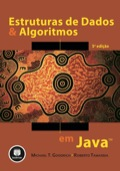
\includegraphics[height=0.3\paperheight]{imagens/livro_goodrich.jpg}
\end{figure}
\end{column}
\begin{column}{0.85\linewidth}
\vspace{3mm}
\textbf{Capítulo 4}\\
\scriptsize{GOODRICH, Michael T.; TAMASSIA, Roberto. \textbf{Estruturas de dados e algoritmos em Java}. Tradução: Bernardo Copstein. 5. ed. Porto Alegre: Bookman, 2013. xxii, 713 p. E-book. ISBN 9788582600191. Tradução de: Data Structures and Algorithms in Java, 5th Edition. Disponível em: \textless{}\url{https://integrada.minhabiblioteca.com.br/\#/books/9788582600191/}\textgreater{}. Acesso em: 01 ago. 2023.}
\end{column}
\end{columns}

\vspace{5mm}

\begin{columns}[T]
\begin{column}{0.15\linewidth}
\vspace{-3mm}
\begin{figure}[h]
	\centering
	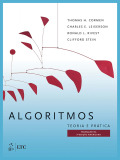
\includegraphics[height=0.3\paperheight]{imagens/livro_cormen.jpg}
\end{figure}
\end{column}
\begin{column}{0.85\linewidth}
\vspace{3mm}
\textbf{Capítulo 3}\\
\scriptsize{CORMEN, Thomas \emph{et al}. \textbf{Algoritmos - Teoria e Prática}. Tradução: Arlete Simille Marques. Rio de Janeiro: Grupo GEN, 2012. E-book. ISBN 9788595158092. Tradução de: Introduction to Algorithms, 3rd ed. Disponível em: \textless{}\url{https://integrada.minhabiblioteca.com.br/\#/books/9788595158092/}\textgreater{}. Acesso em: 01 ago. 2023.}
\end{column}
\end{columns}

\end{frame}

%-------------------------------------------------------
\begin{frame}\frametitle{Sumário}
\begin{itemize}
	\item Complexidade e análise de algoritmos
	\item Medindo o tempo
	\item Contagem de operações
	\item Funções
	\item Exercícios
	\item Notação $O$
	\item Notação $\Omega$ e Notação $\Theta$
	\item Análise assintótica
\end{itemize}
\end{frame}

%=======================================================
\section{Complexidade e análise de algoritmos}

%-------------------------------------------------------
\begin{frame}\frametitle{Complexidade e análise de algoritmos}
\begin{itemize}
	\item  No desenvolvimento de uma aplicação tem-se como objetivo projetar ``boas'' estruturas de dados e ``bons'' algoritmos
	\begin{itemize}
		\item Otimizados
		\item Simples
	\end{itemize}
	\item Como saber se um algoritmo é eficiente?
\end{itemize}
\end{frame}

%-------------------------------------------------------
\begin{frame}\frametitle{Análise de Algoritmos}
\begin{itemize}
	\item Estudo das características de desempenho de um determinado algoritmo
	\begin{itemize}
		\item O espaço ocupado é uma característica de desempenho
		\item O tempo gasto na execução é outra característica de desempenho
	\end{itemize}
\end{itemize}
\end{frame}

%-------------------------------------------------------
\begin{frame}\frametitle{Complexidade de Algoritmos}
\begin{itemize}
	\item A \textbf{complexidade de um algoritmo} é a \textbf{medida do consumo de recursos} de que o algoritmo necessita durante a sua execução
	\begin{itemize}
		\item Tempo de processamento
		\item Memória ocupada
		\item Largura de banda de comunicação
		\item Hardware necessário
		\item etc.
	\end{itemize}
\end{itemize}
\end{frame}

%=======================================================
\section{Medindo o tempo}

%-------------------------------------------------------
\begin{frame}\frametitle{Tempo de processamento}
\begin{itemize}
	\item Depende de uma série de fatores: \emph{hardware}, \emph{software}, tamanho e tipo da entrada de dados
	\item Algoritmo: tempo de execução (ms) X tamanho da entrada de dados (n)
%\vspace{-5mm}
\begin{columns}[T]
\begin{column}{0.5\linewidth}
\begin{figure}[h]
	\centering
	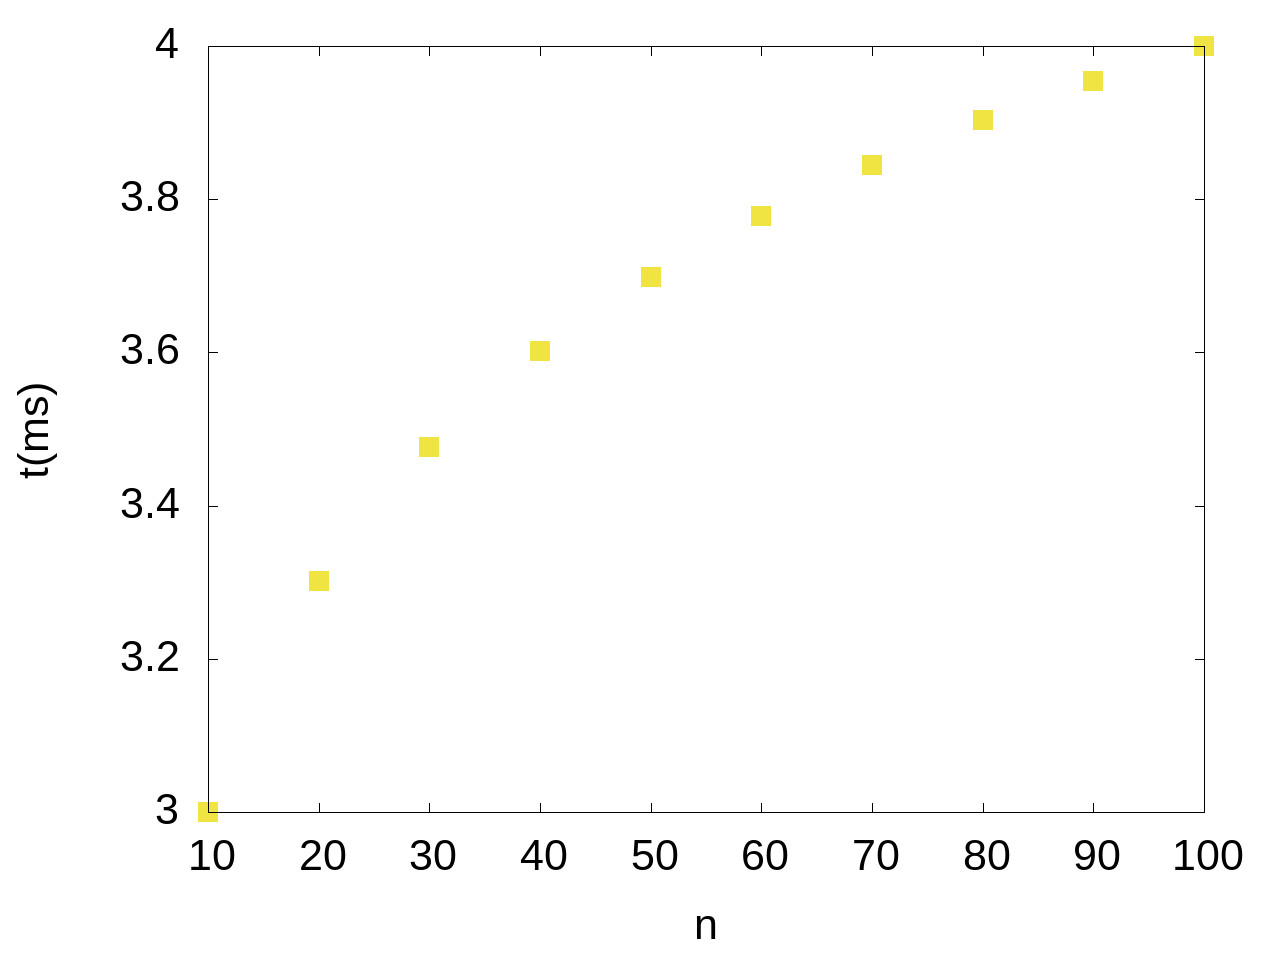
\includegraphics[height=0.6\paperheight]{graficos/grafico.jpg}
\end{figure}
\end{column}
\begin{column}{0.5\linewidth}
\vspace{5mm}
{\fontsize{0}{4}\selectfont{}\textbf{GNUPLOT:}
\verbatiminput{graficos/grafico.gnuplot}
~\\
~\\
\textbf{grafico.txt:}
\verbatiminput{graficos/grafico.txt}
}
\end{column}
\end{columns}

\end{itemize}
\end{frame}

%-------------------------------------------------------
\begin{frame}[fragile]\frametitle{Medindo o tempo}
\begin{itemize}
	\item Em Java, \texttt{System.currentTimeMillis()} retorna o tempo em milissegundos (ms)
{\scriptsize
\begin{lstlisting}
long antes = System.currentTimeMillis();
// algoritmo a ser medido...
long ms = System.currentTimeMillis() - antes;
\end{lstlisting}}
	\item Em Java, \texttt{System.nanoTime()} retorna o tempo em nanossegundos (ns)
{\scriptsize
\begin{lstlisting}
long antes = System.nanoTime();
// algoritmo a ser medido...
long ns = System.nanoTime() - antes;
\end{lstlisting}}
	\item Em C, no Unix, pode-se usar \texttt{gettimeofday()} (incluir \texttt{<sys/time.h>})
{\scriptsize\begin{lstlisting}
struct timeval antes, depois;
gettimeofday(&antes, NULL);
// algoritmo a ser medido...
gettimeofday(&depois, NULL);
unsigned long us = (depois.tv_sec  - antes.tv_sec) * 1000000 +
                   depois.tv_usec - antes.tv_usec;
\end{lstlisting}}

\end{itemize}
\end{frame}

%-------------------------------------------------------
\begin{frame}[fragile]\frametitle{Exemplo: Pesquisa Linear}
\begin{itemize}
	\item A função abaixo recebe um arranjo, o seu tamanho e um valor a ser localizado, e retorna a posição do valor no arranjo (ou -1 se não achar)
{\small\lstinputlisting{pesquisa_linear/pesquisa_linear.c}}
	\item Melhor caso: o valor procurado é o primeiro elemento do arranjo
	\item Pior caso: o valor procurado NÃO existe no arranjo
	\item O arranjo precisa estar ordenado?\\
	\pause
	\textbf{NÃO}
\end{itemize}
\end{frame}

%-------------------------------------------------------
\begin{frame}[fragile]\frametitle{Exemplo: Pesquisa Linear}
\begin{itemize}
	\item Para visualizar como o algoritmo se comporta (``entender'' a sua complexidade), executa-se a função com valores crescentes de arranjo
{\fontsize{0}{5.5}\selectfont\lstinputlisting{pesquisa_linear/main.c}}
\end{itemize}
\end{frame}

%-------------------------------------------------------
\begin{frame}[fragile]\frametitle{Exemplo: Pesquisa Linear (Resultado)}
\vspace{-5mm}
\begin{columns}[T]
\begin{column}{0.1\linewidth}{\tiny
\verbatiminput{pesquisa_linear/curva-inicio.txt}
}
\end{column}
\begin{column}{0.55\linewidth}
\begin{figure}[h]
	\centering
	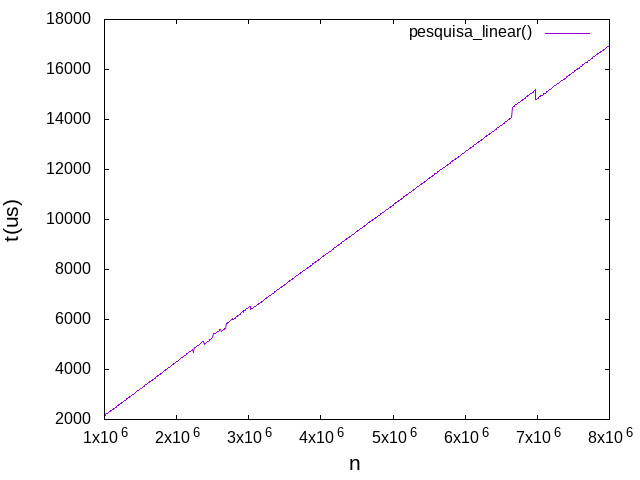
\includegraphics[height=0.65\paperheight]{pesquisa_linear/grafico.jpg}
\end{figure}
\end{column}
\begin{column}{0.35\linewidth}
\vspace{5mm}
{\fontsize{0}{4}\selectfont{}\textbf{GNUPLOT:}
\verbatiminput{pesquisa_linear/grafico.gnuplot}
}
\end{column}
\end{columns}
\end{frame}

%-------------------------------------------------------
\begin{frame}[fragile]\frametitle{Exemplo: Pesquisa Linear (Considerações)}
\begin{itemize}
	\item Considerando o algoritmo e a sua implementação, que tipo de curva de desempenho seria possível esperar?
	\item É possível visualizar a curva esperada no gráfico obtido?
	\item Qual a origem das variações do tempo de execução?
\end{itemize}
\end{frame}

%-------------------------------------------------------
\begin{frame}[fragile]\frametitle{Exercício 1: \emph{Bubble Sort} (Linux)}
\begin{itemize}
	\item Implemente o algoritmo de ordenação \emph{BubbleSort}, por exemplo, a partir do pseudocódigo disponível na Wikipedia (\url{https://pt.wikipedia.org/wiki/Bubble_sort}) -- use o seguinte protótipo como modelo:
{\scriptsize
\begin{lstlisting}
void bubble_sort(int *dados, int tam);
\end{lstlisting}}
	\item Acrescente a sua implementação ao código da próxima página
	\begin{itemize}
		\item Este código trabalha com $n$ variando de 1000 até 10000 com incremento 10, e medindo o tempo em microssegundos
	\end{itemize}
	\item Gere o gráfico de desempenho a partir da execução
	\begin{itemize}
		\item Salve seu código em um arquivo chamado \texttt{bubble\_sort.c} e compile-o usando:\\
		\texttt{gcc -o bubble\_sort bubble\_sort.c}
		\item Execute o programa direcionando a sua saída para um arquivo chamado \texttt{curva1.txt}:\\
		\texttt{./bubble\_sort \textgreater curva1.txt}
		\item Use o \textbf{GNUPLOT} para visualizar o arquivo \texttt{curva1.txt} (dicas nas próximas páginas)
	\end{itemize}
\end{itemize}
\end{frame}

%-------------------------------------------------------
\begin{frame}[fragile]\frametitle{Exercício 1: \emph{Bubble Sort} (código da função \texttt{main()})}
{\fontsize{0}{5.4}\selectfont\lstinputlisting{bubble_sort/main.c}}
\end{frame}

%-------------------------------------------------------
\begin{frame}[fragile]\frametitle{Exercício 1: \emph{Bubble Sort} (dicas sobre \textbf{GNUPLOT})}
\begin{itemize}
	\item \textbf{GNUPLOT} é um aplicativo para gerar gráficos, disponível em várias plataformas
	\item Para mostrar, por exemplo, o gráfico correspondente aos dados armazenados no arquivo \texttt{curva1.txt} em uma janela, executa-se o \textbf{GNUPLOT} (\texttt{gnuplot}) e digita-se os seguintes comandos:
{\scriptsize
\begin{verbatim}
set xlabel "n" font "Arial,16"
set ylabel "t(us)" font "Arial,16"
plot "curva1.txt" with lines title "bubble\\_sort()"
\end{verbatim}
}
	\item Para gerar um arquivo JPEG com o conteúdo do gráfico, pode-se usar os seguintes comandos:
{\scriptsize
\begin{verbatim}
set terminal jpeg
set output "grafico1.jpg"
set xlabel "n" font "Arial,16"
set ylabel "t(us)" font "Arial,16"
plot "curva1.txt" with lines title "bubble\\_sort()"
\end{verbatim}
}
\end{itemize}
\end{frame}

%-------------------------------------------------------
\begin{frame}[fragile]\frametitle{Solução 1: \emph{Bubble Sort} (primeira implementação)}
{\scriptsize\lstinputlisting{bubble_sort/bubble_sort1.c}}
\end{frame}

%-------------------------------------------------------
\begin{frame}[fragile]\frametitle{Solução 1: \emph{Bubble Sort} (gráfico da primeira implementação)}
\vspace{-5mm}
\begin{columns}[T]
\begin{column}{0.6\linewidth}
\begin{figure}[h]
	\centering
	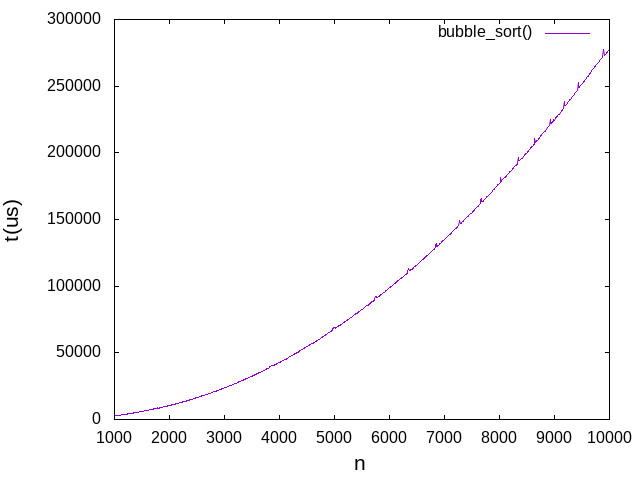
\includegraphics[height=0.75\paperheight]{bubble_sort/grafico1.jpg}
\end{figure}
\end{column}
\begin{column}{0.4\linewidth}
\vspace{5mm}
{\fontsize{0}{4}\selectfont{}\textbf{GNUPLOT:}
\verbatiminput{bubble_sort/grafico1.gnuplot}
}
\end{column}
\end{columns}
\end{frame}

%-------------------------------------------------------
\begin{frame}[fragile]\frametitle{Exercício 2: \emph{Bubble Sort} otimizado}
\begin{itemize}
	\item A versão sugerida para implementação do \emph{Bubble Sort} tem um problema:
	\begin{itemize}
		\item Depois de executar uma passagem, o maior elemento é ``empurrado'' para a sua posição
		\item E: as passagens seguintes continuam ``tentado'' empurrar o maior elemento para o final
	\end{itemize}
	\item A solução consiste em diminuir gradualmente o tamanho até onde cada passagem é executada
	\item Implemente esta solução e compare o seu desempenho com a versão anterior
\end{itemize}
\end{frame}

%-------------------------------------------------------
\begin{frame}[fragile]\frametitle{Solução 2: \emph{Bubble Sort} otimizado}
{\scriptsize\lstinputlisting{bubble_sort/bubble_sort2.c}}
\end{frame}

%-------------------------------------------------------
\begin{frame}[fragile]\frametitle{Solução 2: \emph{Bubble Sort} otimizado (comandos do \texttt{gnuplot})}
\begin{verbatim}
set xlabel "n" font "Arial,16"
set ylabel "t(us)" font "Arial,16"
plot "curva1.txt" with lines title "Bubble Sort",
     "curva2.txt" with lines title "Bubble Sort Otimizado"
\end{verbatim}
\end{frame}

%-------------------------------------------------------
\begin{frame}[fragile]\frametitle{Solução 2: \emph{Bubble Sort} (gráfico das duas implementações)}
\vspace{-5mm}
\begin{columns}[T]
\begin{column}{0.6\linewidth}
\begin{figure}[h]
	\centering
	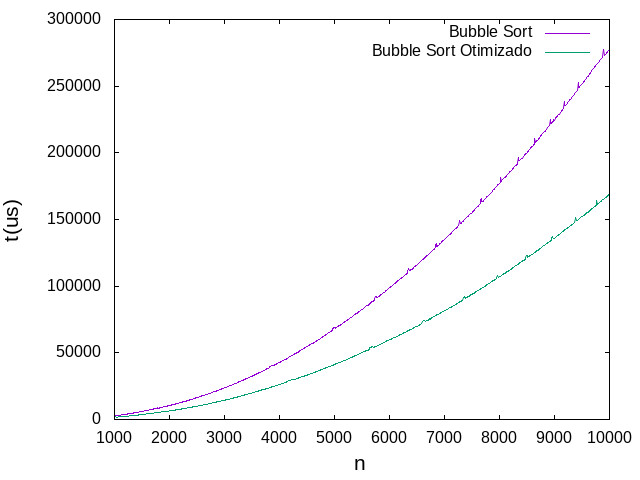
\includegraphics[height=0.75\paperheight]{bubble_sort/grafico2.jpg}
\end{figure}
\end{column}
\begin{column}{0.4\linewidth}
\vspace{5mm}
{\fontsize{0}{4}\selectfont{}\textbf{GNUPLOT:}
\verbatiminput{bubble_sort/grafico2.gnuplot}
}
\end{column}
\end{columns}
\end{frame}

%-------------------------------------------------------
\begin{frame}\frametitle{Análise da eficiência de um algoritmo}
\begin{itemize}
	\item Medir o tempo depende de hardware e software (sistema operacional, por exemplo)
	\item Alternativa?\\
	\pause
	\textbf{Contar o número de operações (atribuição, operação aritmética, comparação, etc.)}
\end{itemize}
\end{frame}

%=======================================================
\section{Contagem de operações}

%-------------------------------------------------------
\begin{frame}\frametitle{Análise de algoritmos}
\begin{itemize}
	\item Não considera o tempo de execução
	\item Pode ser feita diretamente sobre o pseudocódigo de alto nível
	\item Consiste em contar quantas \textbf{operações primitivas} são executadas
	\begin{itemize}
		\item Operação primitiva: instrução de baixo nível com um tempo de execução constante
	\end{itemize}
	\item Assume-se que os tempos de execução de operações primitivas diferentes são similares
\end{itemize}
\end{frame}

%-------------------------------------------------------
\begin{frame}\frametitle{Operações primitivas}
\begin{itemize}
	\item Atribuição de valores a variáveis
	\item Chamadas de métodos
	\item Operações aritméticas (por exemplo, adição de dois números)
	\item Comparação de dois números
	\item Acesso a um arranjo
	\item Retorno de um método
\end{itemize}
\end{frame}

%-------------------------------------------------------	
\begin{frame}[fragile]\frametitle{Exemplo 1}
\begin{itemize}
	\item Contar o número de operações para atribuir para cada posição v[i] de um arranjo unidimensional o resultado de i*2
\begin{verbatim}
v[0..10] : inteiro
for (i = 0; i < v.comprimento; i++)
    v[i] = i * 2
\end{verbatim}
	\pause
	\item Operação (multiplicação, atribuição e acesso às posições do arranjo): \textbf{$n$}
	\pause
\vspace{-3mm}
\begin{columns}[T]
\begin{column}{0.6\linewidth}
\begin{figure}[h]
	\centering
	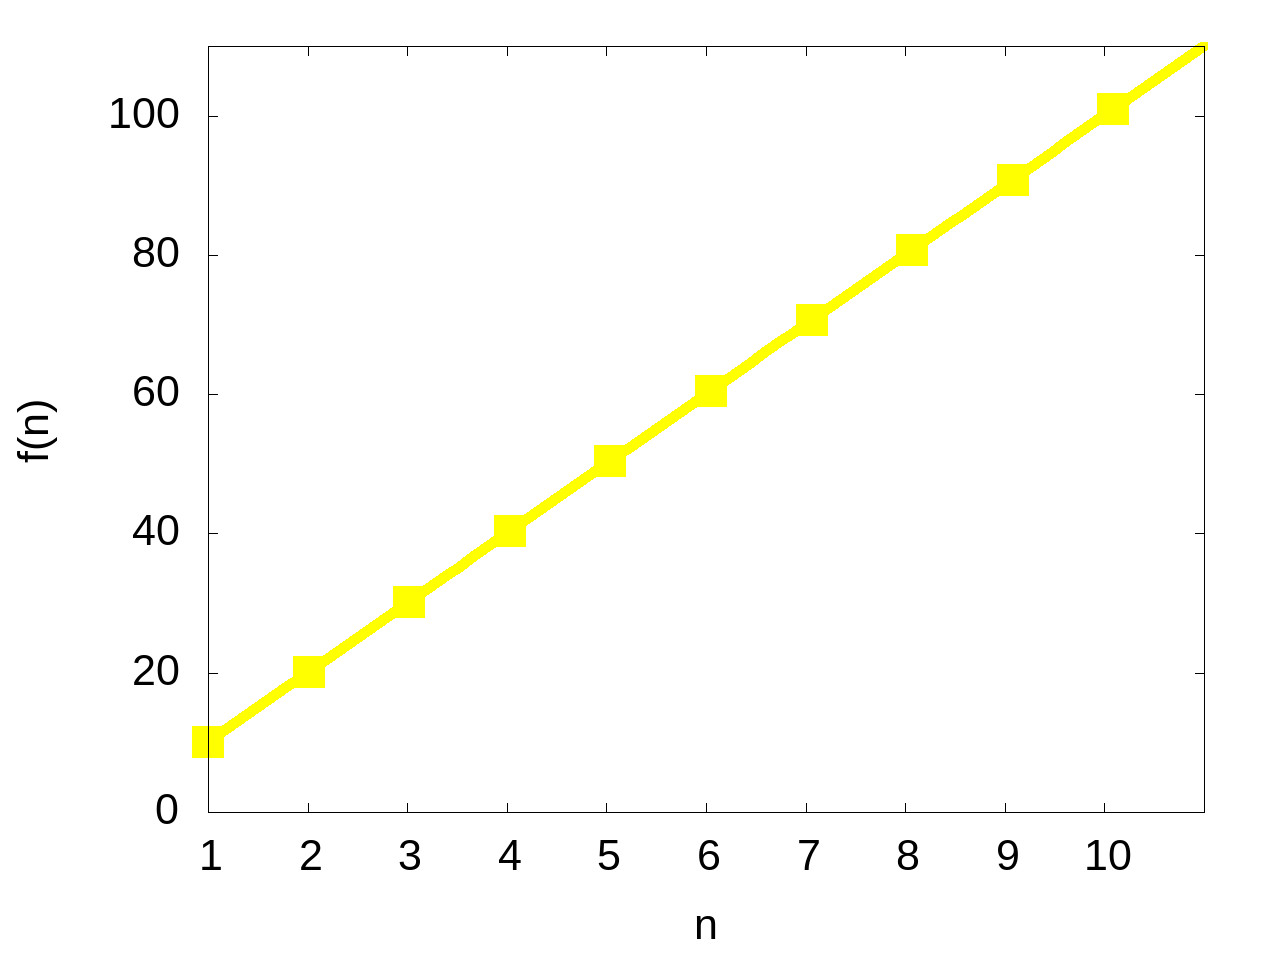
\includegraphics[height=0.4\paperheight]{graficos/10n.jpg}
\end{figure}
\end{column}
\begin{column}{0.4\linewidth}
\vspace{5mm}
{\fontsize{0}{4}\selectfont{}\textbf{GNUPLOT:}
\verbatiminput{graficos/10n.gnuplot}
}
\end{column}
\end{columns}
\end{itemize}
\end{frame}

%-------------------------------------------------------
\begin{frame}[fragile]\frametitle{Exemplo 2}
\begin{itemize}
	\item Contar o número de operações para atribuir para cada posição m[i,j] de um arranjo bidimensional o resultado de i*j
\begin{verbatim}
m[0..10][0..10] : inteiro
for (i=0; i<m.comprimento; i++)
    for (j=0; j<m[i].comprimento; j++)
        m[i][j] = i * j
\end{verbatim}
	\pause
	\item Operação (multiplicação, atribuição e acesso às posições do arranjo): \textbf{$n \times n$}
	\pause
\vspace{-3mm}
\begin{columns}[T]
\begin{column}{0.6\linewidth}
\begin{figure}[h]
	\centering
	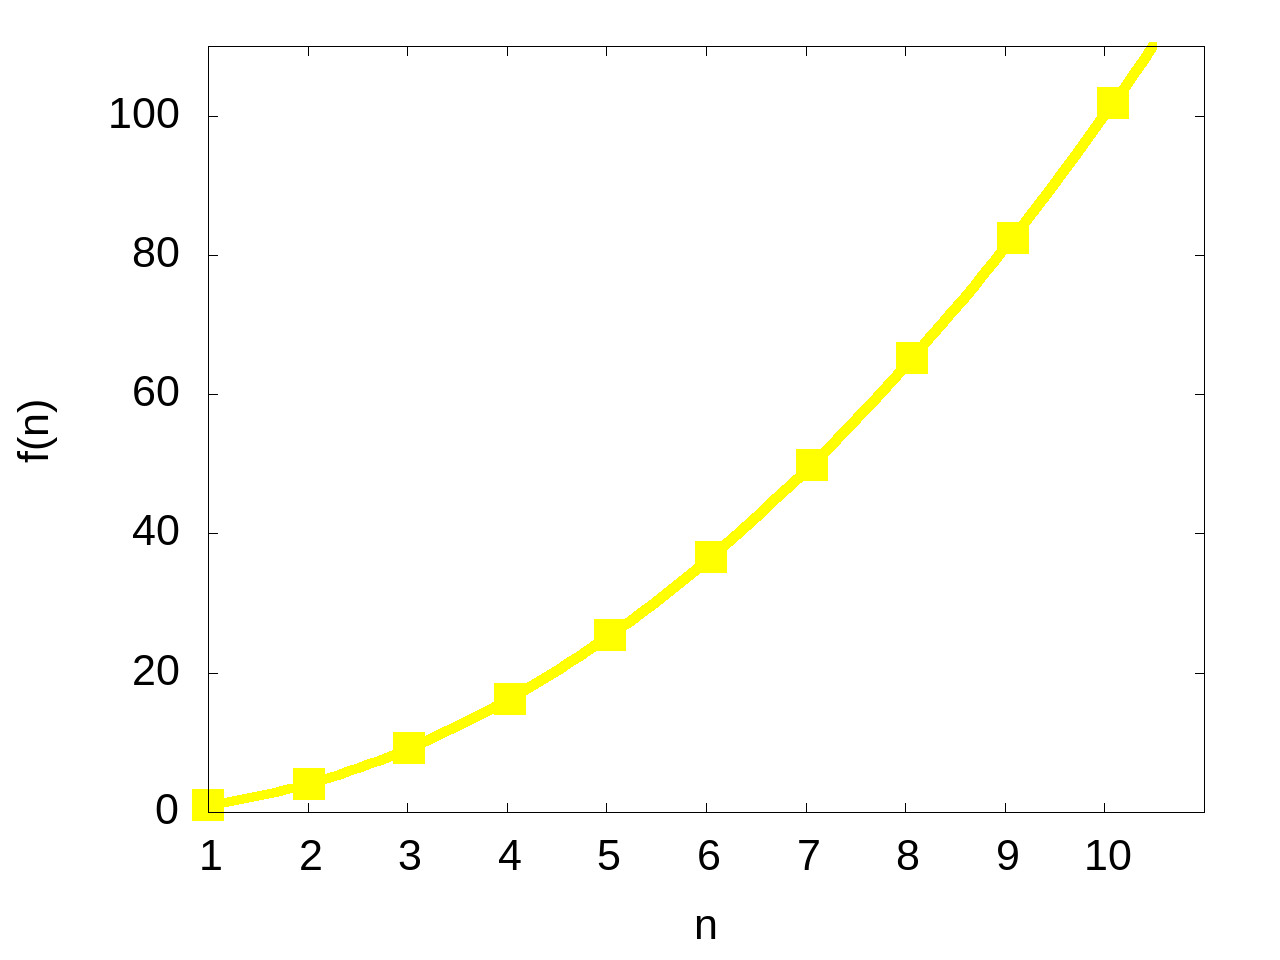
\includegraphics[height=0.35\paperheight]{graficos/nxn.jpg}
\end{figure}
\end{column}
\begin{column}{0.4\linewidth}
\vspace{5mm}
{\fontsize{0}{4}\selectfont{}\textbf{GNUPLOT:}
\verbatiminput{graficos/nxn.gnuplot}
}
\end{column}
\end{columns}
\end{itemize}
\end{frame}

%-------------------------------------------------------
\begin{frame}[fragile]\frametitle{Exercício (1/2)}
Conte o número de operações executadas pelas seguintes funções.
\begin{columns}[T]
\begin{column}{0.5\linewidth}
\begin{enumerate}
	\item {\scriptsize\lstinputlisting{contagem/contagem01.c}}
	\item {\scriptsize\lstinputlisting{contagem/contagem02.c}}
\end{enumerate}
\end{column}
\begin{column}{0.5\linewidth}
\begin{enumerate}
	\setcounter{enumi}{2}
	\item {\scriptsize\lstinputlisting{contagem/contagem03.c}}
	\item {\scriptsize\lstinputlisting{contagem/contagem04.c}}
\end{enumerate}
\end{column}
\end{columns}
\end{frame}

%-------------------------------------------------------
\begin{frame}[fragile]\frametitle{Exercício (2/2)}
\begin{enumerate}
	\setcounter{enumi}{4}
	\item {\scriptsize\lstinputlisting{contagem/contagem05.c}}
	\item {\scriptsize\lstinputlisting{contagem/contagem06.c}}
\end{enumerate}
\end{frame}

%-------------------------------------------------------
\begin{frame}[fragile]\frametitle{Exercício: soluções (1/6)}
\begin{columns}[T]
\begin{column}{0.5\linewidth}
%\vspace{-4mm}
\begin{enumerate}
	\setcounter{enumi}{0}
	\item {\scriptsize\lstinputlisting{contagem/contagem01.c}}
{\tiny
\begin{verbatim}
n = 10   /  i = 0..9    [op = 10]

n = 20   /  i = 0..19   [op = 20]

n = 50   /  i = 0..49   [op = 50]

n = 100  /  i = 0..99   [op = 100]

n = 1000 /  i = 0..999  [op = 1000]
\end{verbatim}
Número de operações: $n \therefore O(n)$
}
\end{enumerate}
\end{column}
\begin{column}{0.5\linewidth}
\begin{figure}[h]
	\centering
		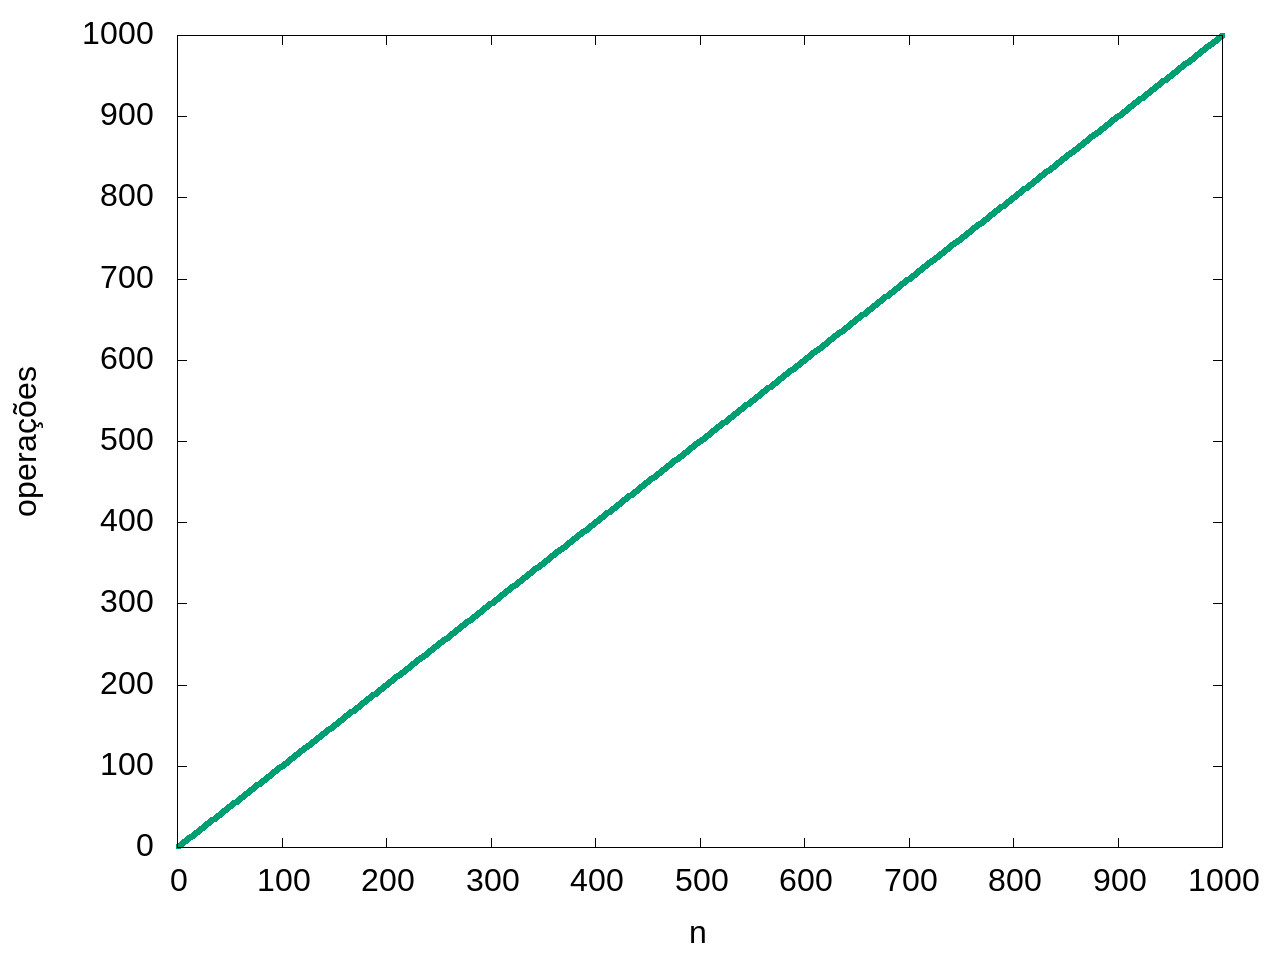
\includegraphics[height=0.5\paperheight]{contagem/contagem01.jpg}
\end{figure}
{\fontsize{0}{4}\selectfont{}\textbf{GNUPLOT:}
\verbatiminput{contagem/contagem01.gnuplot}
}
\end{column}
\end{columns}
\end{frame}

%-------------------------------------------------------
\begin{frame}[fragile]\frametitle{Exercício: soluções (2/6)}
\begin{columns}[T]
\begin{column}{0.5\linewidth}
%\vspace{-4mm}
\begin{enumerate}
	\setcounter{enumi}{1}
	\item {\scriptsize\lstinputlisting{contagem/contagem02.c}}
{\tiny
\begin{verbatim}
n = 10  /  i = 0  /  j = 0..9
           i = 1  /  j = 0..9
           i = 2  /  j = 0..9
           i = 3  /  j = 0..9
           i = 4  /  j = 0..9
           i = 5  /  j = 0..9
           i = 6  /  j = 0..9
           i = 7  /  j = 0..9
           i = 8  /  j = 0..9
           i = 9  /  j = 0..9  [op = 100]
\end{verbatim}
Número de operações: $n \times n = n^{2} \therefore O(n^2)$
}
\end{enumerate}
\end{column}
\begin{column}{0.5\linewidth}
\begin{figure}[h]
	\centering
	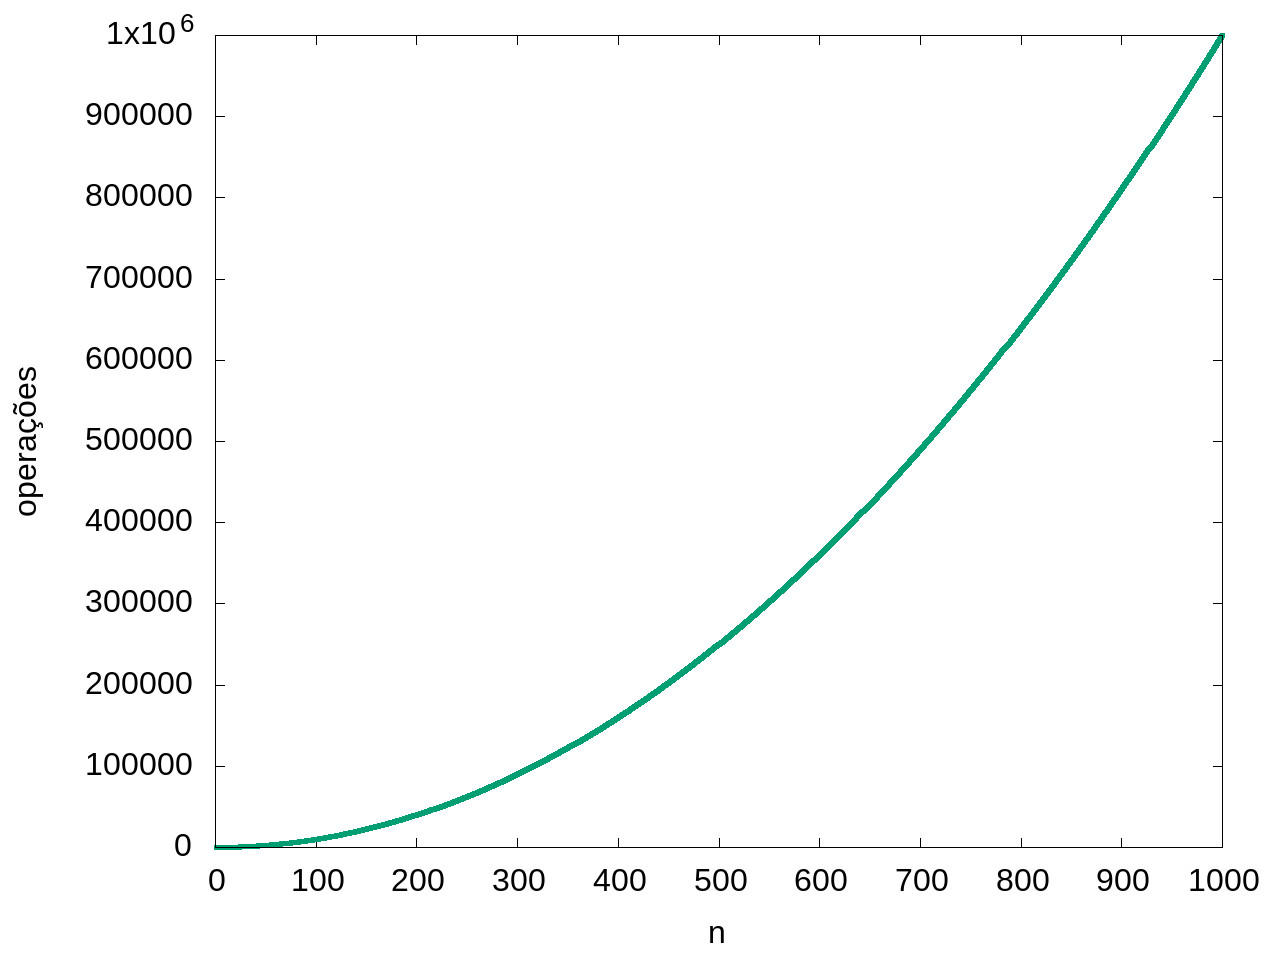
\includegraphics[height=0.5\paperheight]{contagem/contagem02.jpg}
\end{figure}
{\fontsize{0}{4}\selectfont{}\textbf{GNUPLOT:}
\verbatiminput{contagem/contagem02.gnuplot}
}
\end{column}
\end{columns}
\end{frame}

%-------------------------------------------------------
\begin{frame}[fragile]\frametitle{Exercício: soluções (3/6)}
\begin{columns}[T]
\begin{column}{0.5\linewidth}
%\vspace{-4mm}
\begin{enumerate}
	\setcounter{enumi}{2}
	\item {\scriptsize\lstinputlisting{contagem/contagem03.c}}
{\tiny
\begin{verbatim}
n = 10  /  i = 0  /  j = 1,2,3,4,5,6,7,8,9
           i = 1  /  j = 2,3,4,5,6,7,8,9
           i = 2  /  j = 3,4,5,6,7,8,9
           i = 3  /  j = 4,5,6,7,8,9
           i = 4  /  j = 5,6,7,8,9
           i = 5  /  j = 6,7,8,9
           i = 6  /  j = 7,8,9
           i = 7  /  j = 8,9
           i = 8  /  j = 9
           i = 9  /  j =        [op = 45]
\end{verbatim}
Número de operações: $\frac{n \times (n-1)}{2} = \frac{n^2}{2}-\frac{n}{2} \therefore O(n^2)$
}
\end{enumerate}	
\end{column}
\begin{column}{0.5\linewidth}
\begin{figure}[h]
	\centering
	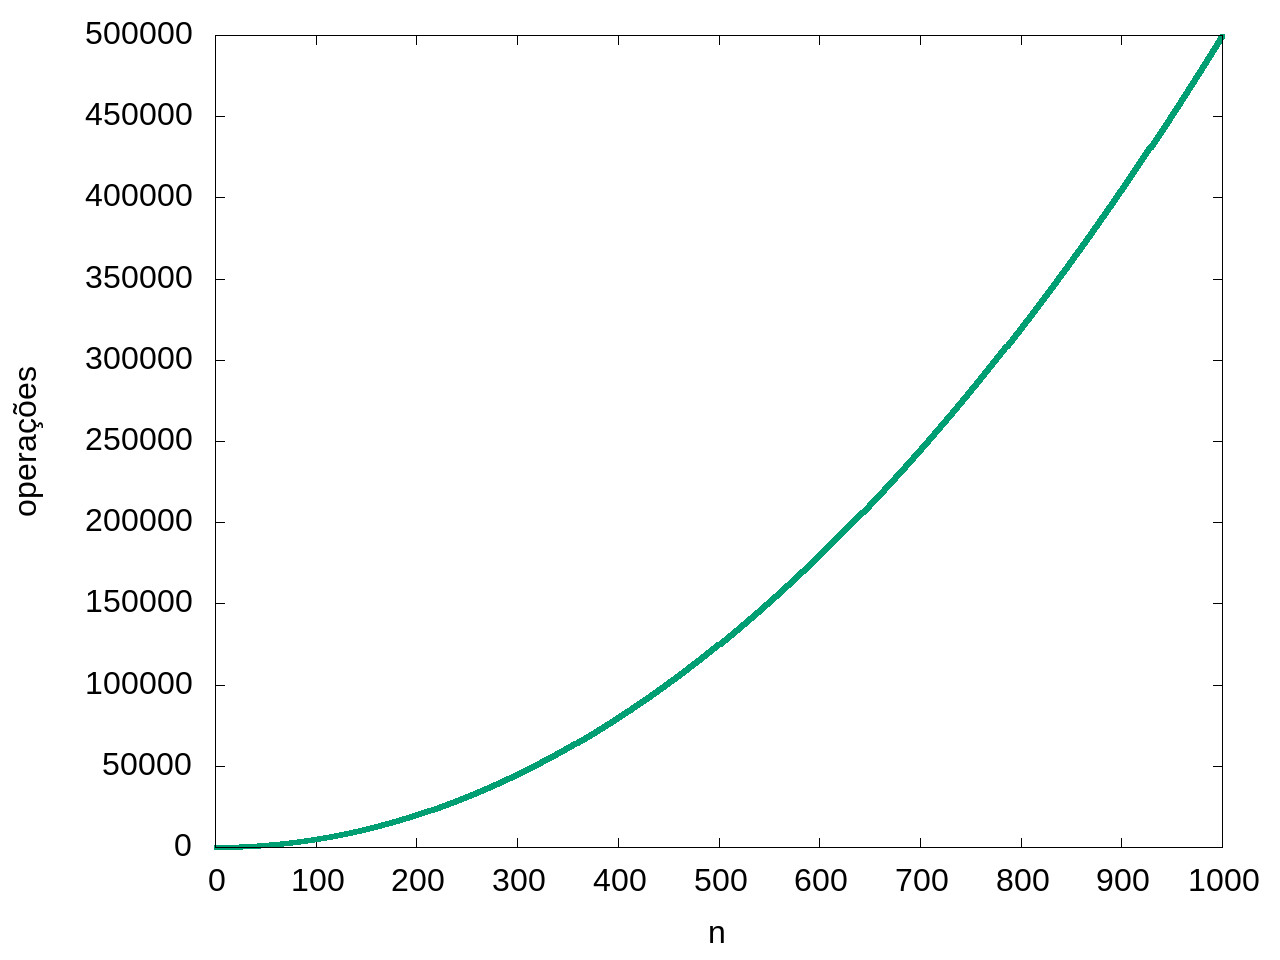
\includegraphics[height=0.5\paperheight]{contagem/contagem03.jpg}
\end{figure}
{\fontsize{0}{4}\selectfont{}\textbf{GNUPLOT:}
\verbatiminput{contagem/contagem03.gnuplot}
}
\end{column}
\end{columns}
\end{frame}

\begin{comment}
int f4(n)
    r=0
    for (i=1; i<n; i++)
        for (j=i; j<2*i; j++)
            for (k=i; k<j; k++)
                r = r + 1
     return r
\end{comment}

%-------------------------------------------------------
\begin{frame}[fragile]\frametitle{Exercício: soluções (4/6)}
\begin{columns}[T]
\begin{column}{0.5\linewidth}
%\vspace{-4mm}
\begin{enumerate}
	\setcounter{enumi}{3}
	\item {\scriptsize\lstinputlisting{contagem/contagem04.c}}
{\tiny
\begin{verbatim}
n = 10  /  i = 0  /  j = 
           i = 1  /  j = 0..1
           i = 2  /  j = 0..3
           i = 3  /  j = 0..5
           i = 4  /  j = 0..7
           i = 5  /  j = 0..9
           i = 6  /  j = 0..11
           i = 7  /  j = 0..13
           i = 8  /  j = 0..15
           i = 9  /  j = 0..17  [op = 90]
\end{verbatim}
Número de operações: $n \times (n-1) = n^2 - n \therefore O(n^2)$
}
\end{enumerate}
\end{column}
\begin{column}{0.5\linewidth}
\begin{figure}[h]
	\centering
	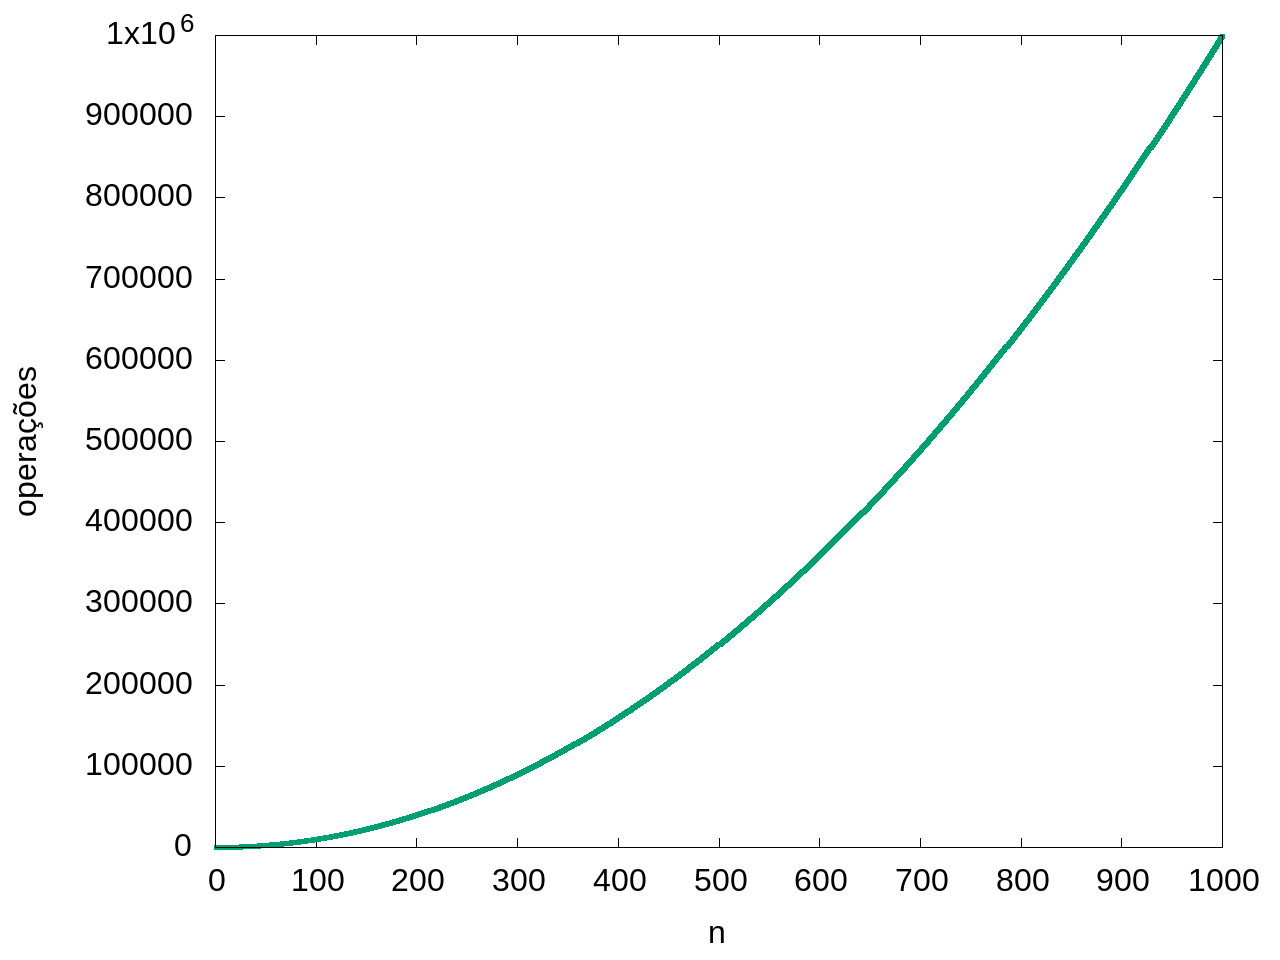
\includegraphics[height=0.5\paperheight]{contagem/contagem04.jpg}
\end{figure}
{\fontsize{0}{4}\selectfont{}\textbf{GNUPLOT:}
\verbatiminput{contagem/contagem04.gnuplot}
}
\end{column}
\end{columns}
\end{frame}

%-------------------------------------------------------
\begin{frame}[fragile]\frametitle{Exercício: soluções (5/6)}
\begin{columns}[T]
\begin{column}{0.5\linewidth}
%\vspace{-4mm}
\begin{enumerate}
	\setcounter{enumi}{4}
	\item {\scriptsize\lstinputlisting{contagem/contagem05.c}}
{\tiny
\begin{verbatim}
n = 10  / i = 0  /  j = 0  /  k = 
                    j = 1  /  k = 0
                    j = 2  /  k = 0..1
          i = 1  /  j = 1  /  k = 
                    j = 2  /  k = 1
                    j = 3  /  k = 1..2
          ...
          i = 9  /  j = 9  /  k = 
                    j = 10 /  k = 9
                    j = 11 /  k = 9..10   [op = 30]
\end{verbatim}
Número de operações: $n \times 3 = 3n \therefore O(n)$
}
\end{enumerate}
\end{column}
\begin{column}{0.5\linewidth}
\begin{figure}[h]
	\centering
	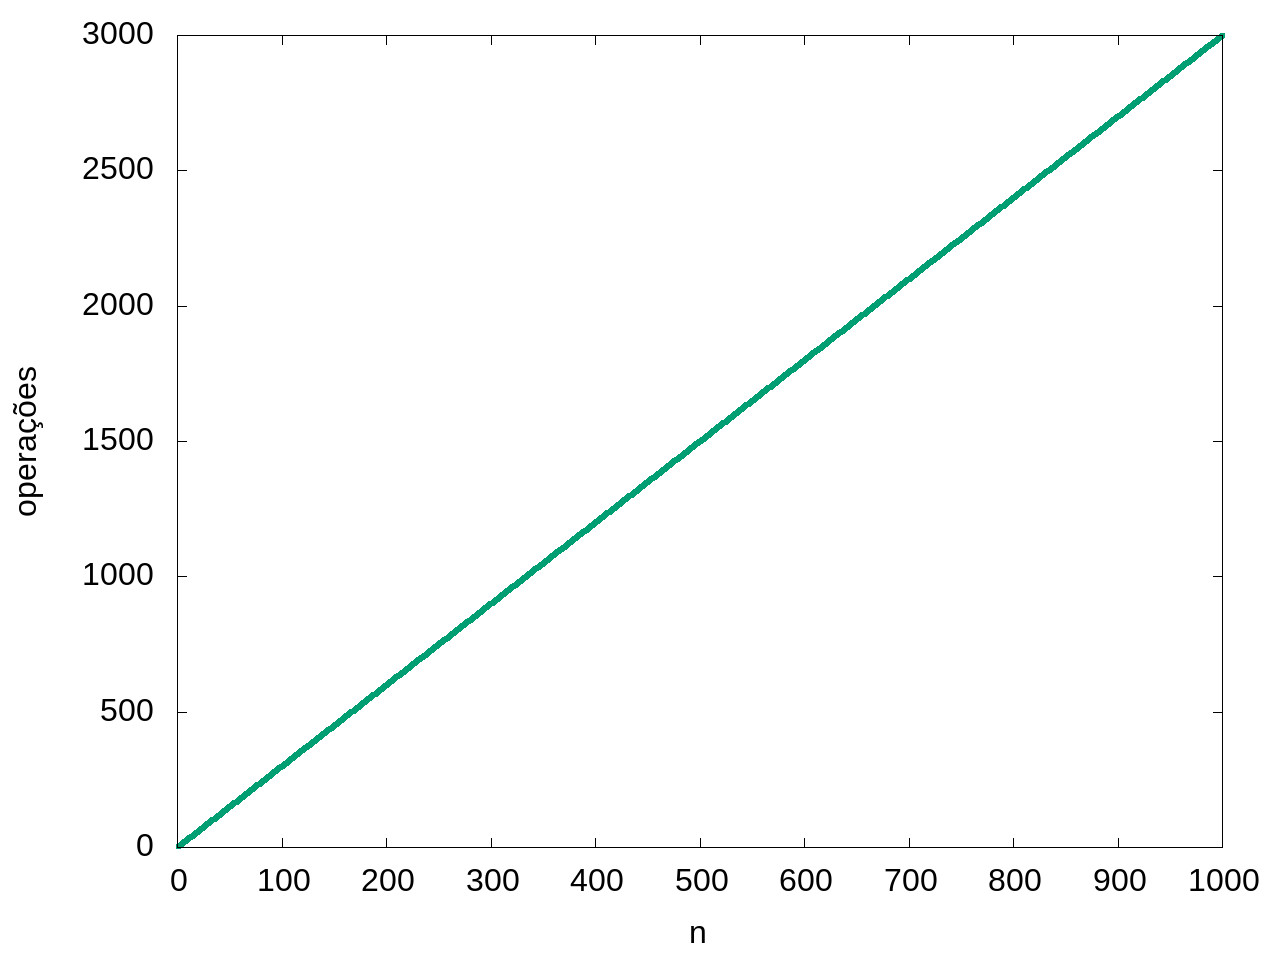
\includegraphics[height=0.5\paperheight]{contagem/contagem05.jpg}
\end{figure}
{\fontsize{0}{4}\selectfont{}\textbf{GNUPLOT:}
\verbatiminput{contagem/contagem05.gnuplot}
}
\end{column}
\end{columns}
\end{frame}

%-------------------------------------------------------
\begin{frame}[fragile]\frametitle{Exercício: soluções (6/6)}
\begin{columns}[T]
\begin{column}{0.5\linewidth}
%\vspace{-4mm}
\begin{enumerate}
	\setcounter{enumi}{5	}
	\item {\scriptsize\lstinputlisting{contagem/contagem06.c}}
{\tiny
\begin{verbatim}
n = 1  [op = 1]	
n = 2  [op = 3]
n = 3  [op = 7]
n = 4  [op = 15]
n = 5  [op = 31]
n = 6  [op = 63]
n = 7  [op = 127]
n = 8  [op = 255]
n = 9  [op = 511]
\end{verbatim}
Número de operações: $2^{n}-1 \therefore O(2^{n})$
}
\end{enumerate}
\end{column}
\begin{column}{0.5\linewidth}
\begin{figure}[h]
	\centering
	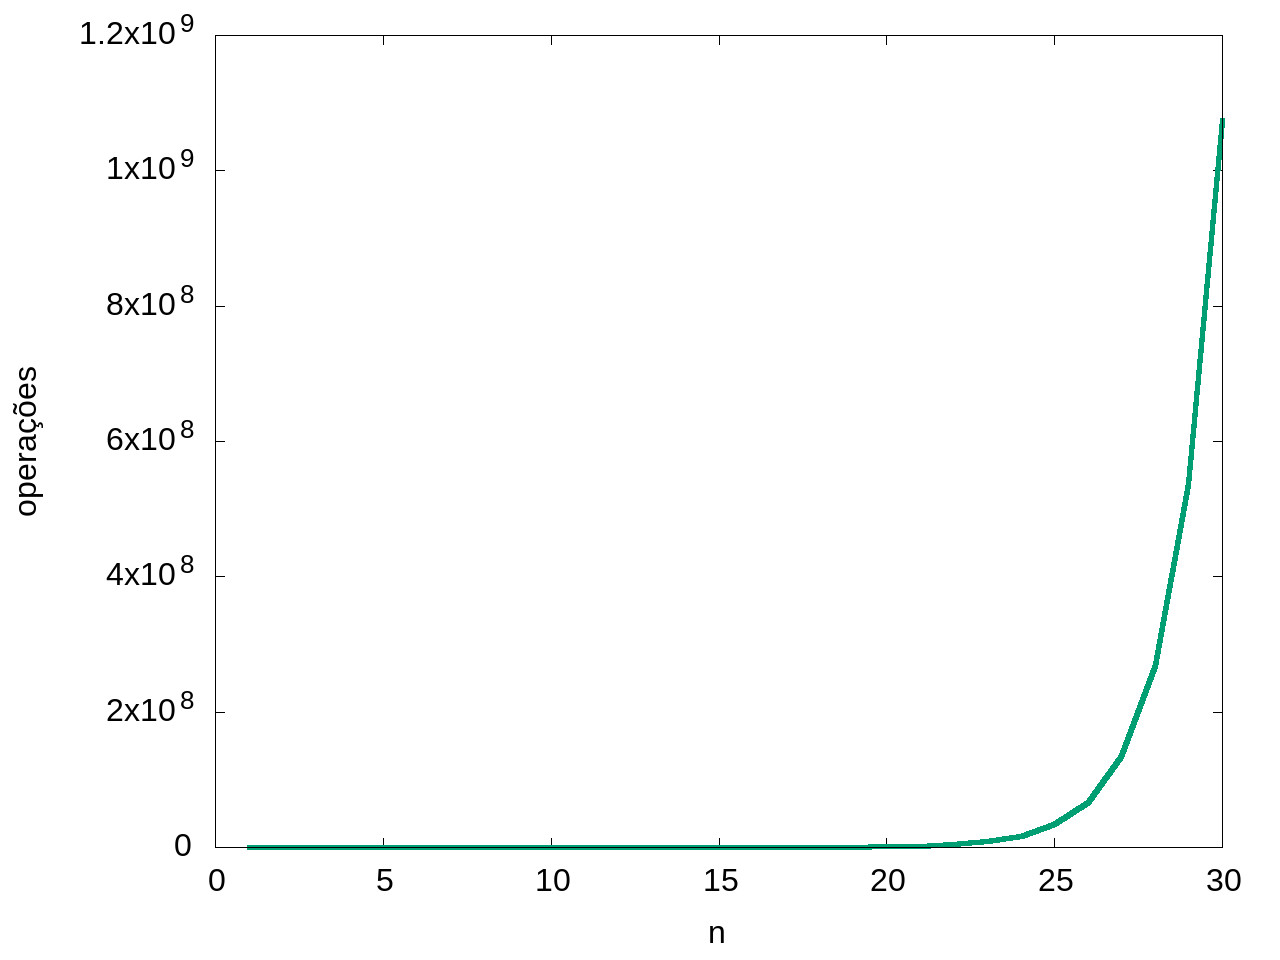
\includegraphics[height=0.5\paperheight]{contagem/contagem06.jpg}
\end{figure}
{\fontsize{0}{4}\selectfont{}\textbf{GNUPLOT:}
\verbatiminput{contagem/contagem06.gnuplot}
}
\end{column}
\end{columns}
\end{frame}

%=======================================================
\section{Funções}

%-------------------------------------------------------
\begin{frame}\frametitle{Funções}
\begin{itemize}
	\item Uma \textbf{classe de complexidade} é uma forma de agrupar algoritmos que apresentam complexidade similar. Por exemplo:
	\begin{itemize}
		\item Complexidade \textbf{constante}: o algoritmo sempre ocupa a mesma quantidade de recursos
		\item Complexidade \textbf{linear}: o algoritmo consome recursos de forma diretamente proporcional ao tamanho do problema
	\end{itemize}
\end{itemize}
\end{frame}

%-------------------------------------------------------
\begin{frame}\frametitle{Funções}
\begin{itemize}
	\item Sete funções mais comuns usadas em análise de algoritmos:
	\begin{itemize}
		\item Constante: $1$
		\item Logaritmo: $\log n$
		\item Linear: $n$
		\item n-log-n: $n \log n$
		\item Quadrática: $n^2$
		\item Cúbica: $n^3$
		\item Exponencial: $a^n$
	\end{itemize}
\end{itemize}
\end{frame}

%-------------------------------------------------------
\begin{frame}\frametitle{Função Constante: $1$}
\begin{itemize}
	\item Função mais simples
	\item $f(n) = c$
	\item Não importa o valor de $n$, sempre será igual ao valor da constante $c$
	\item Exemplo: função que recebe um arranjo de inteiros e retorna o valor do primeiro elemento multiplicado por 2
\end{itemize}
\vspace{-5mm}
\begin{columns}[T]
\begin{column}{0.6\linewidth}
\begin{figure}[h]
	\centering
	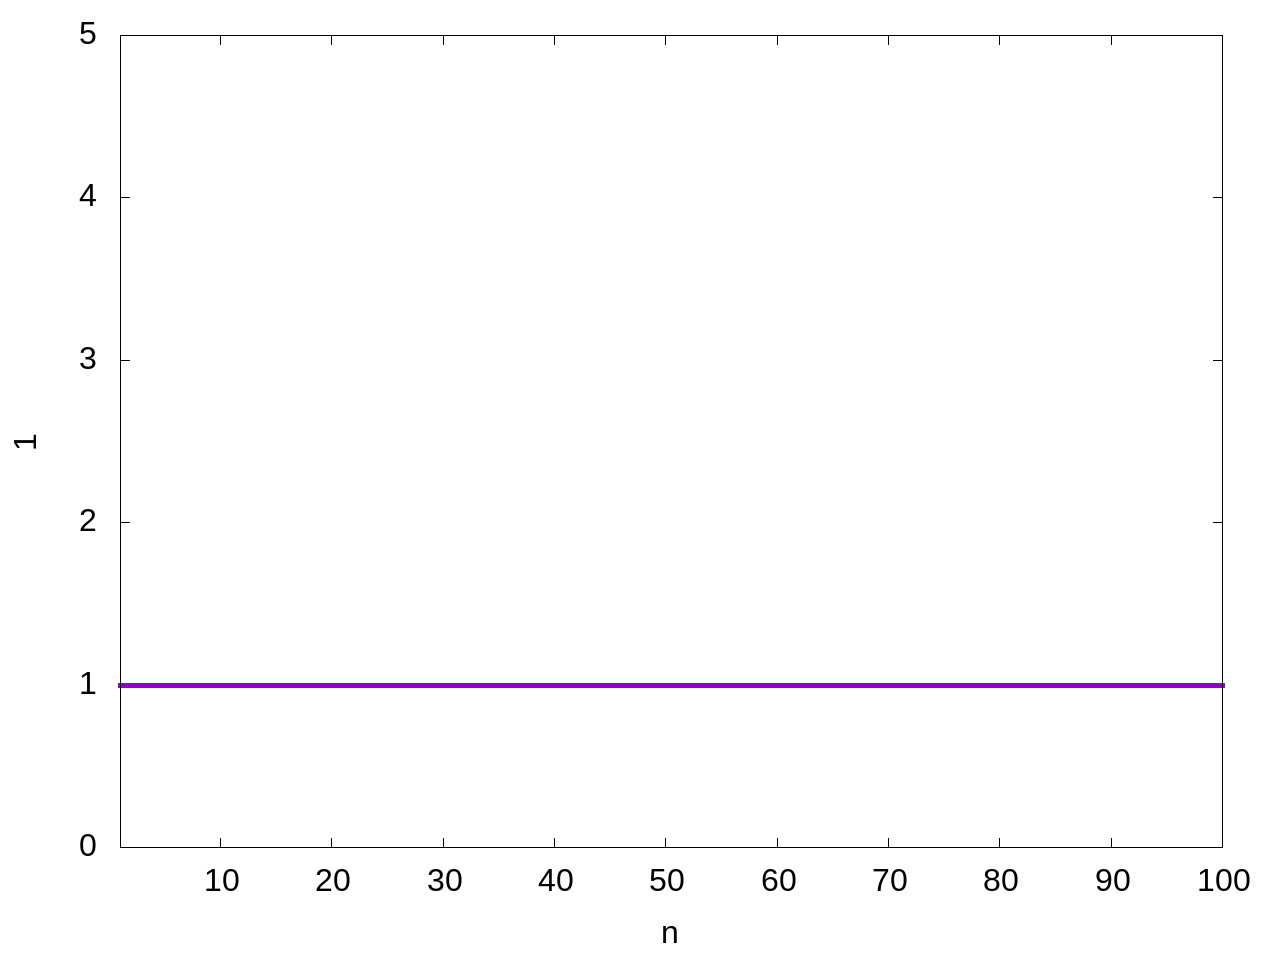
\includegraphics[height=0.5\paperheight]{graficos/1.jpg}
\end{figure}
\end{column}
\begin{column}{0.4\linewidth}
\vspace{5mm}
{\fontsize{0}{4}\selectfont{}\textbf{GNUPLOT:}
\verbatiminput{graficos/1.gnuplot}
}
\end{column}
\end{columns}
\end{frame}

%-------------------------------------------------------
\begin{frame}\frametitle{Função Logaritmo: $\log n$}
\begin{itemize}
	\item $f(n) = \log{}n$ ou $f(n) = \log_{2}n$
	\item O número de operações realizadas para solução do problema não cresce da mesma forma que $n$: se dobra o valor de $n$, o incremento do consumo é bem menor
	\item Exemplo: conversão de número decimal para binário e pesquisa binária (\emph{binary search})
\end{itemize}
\vspace{-5mm}
\begin{columns}[T]
\begin{column}{0.6\linewidth}
\begin{figure}[h]
	\centering
	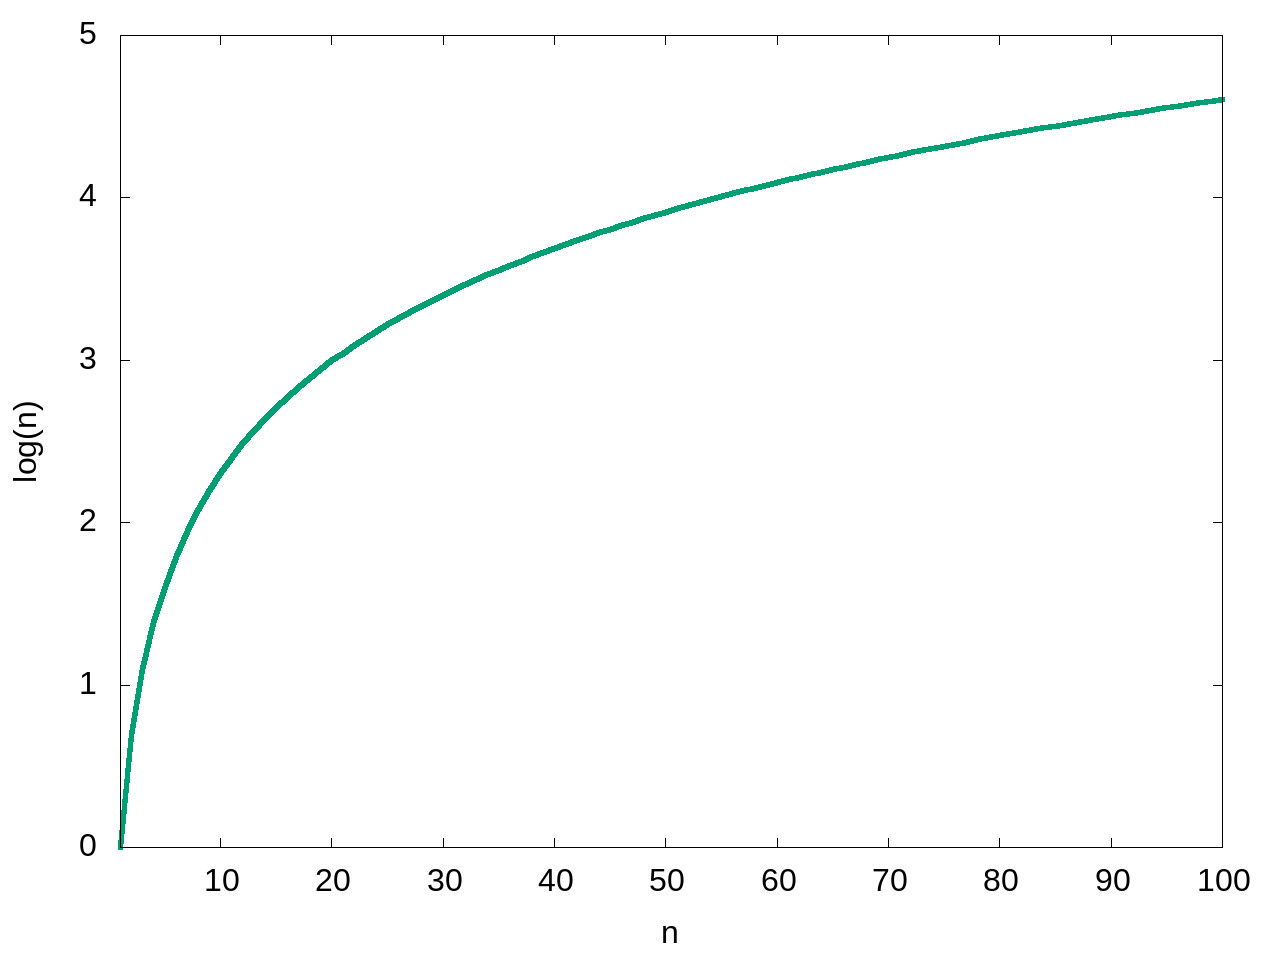
\includegraphics[height=0.5\paperheight]{graficos/log_n.jpg}
\end{figure}
\end{column}
\begin{column}{0.4\linewidth}
\vspace{5mm}
{\fontsize{0}{4}\selectfont{}\textbf{GNUPLOT:}
\verbatiminput{graficos/log_n.gnuplot}
}
\end{column}
\end{columns}
\end{frame}

%-------------------------------------------------------
\begin{frame}\frametitle{Função Linear: $n$}
\begin{itemize}
	\item Se dobra o valor de $n$, dobra o consumo de recursos
	\item $f(n) = n$
	\item Exemplo: localizar um elemento em uma lista
\end{itemize}
\vspace{-5mm}
\begin{columns}[T]
\begin{column}{0.6\linewidth}
\begin{figure}[h]
	\centering
	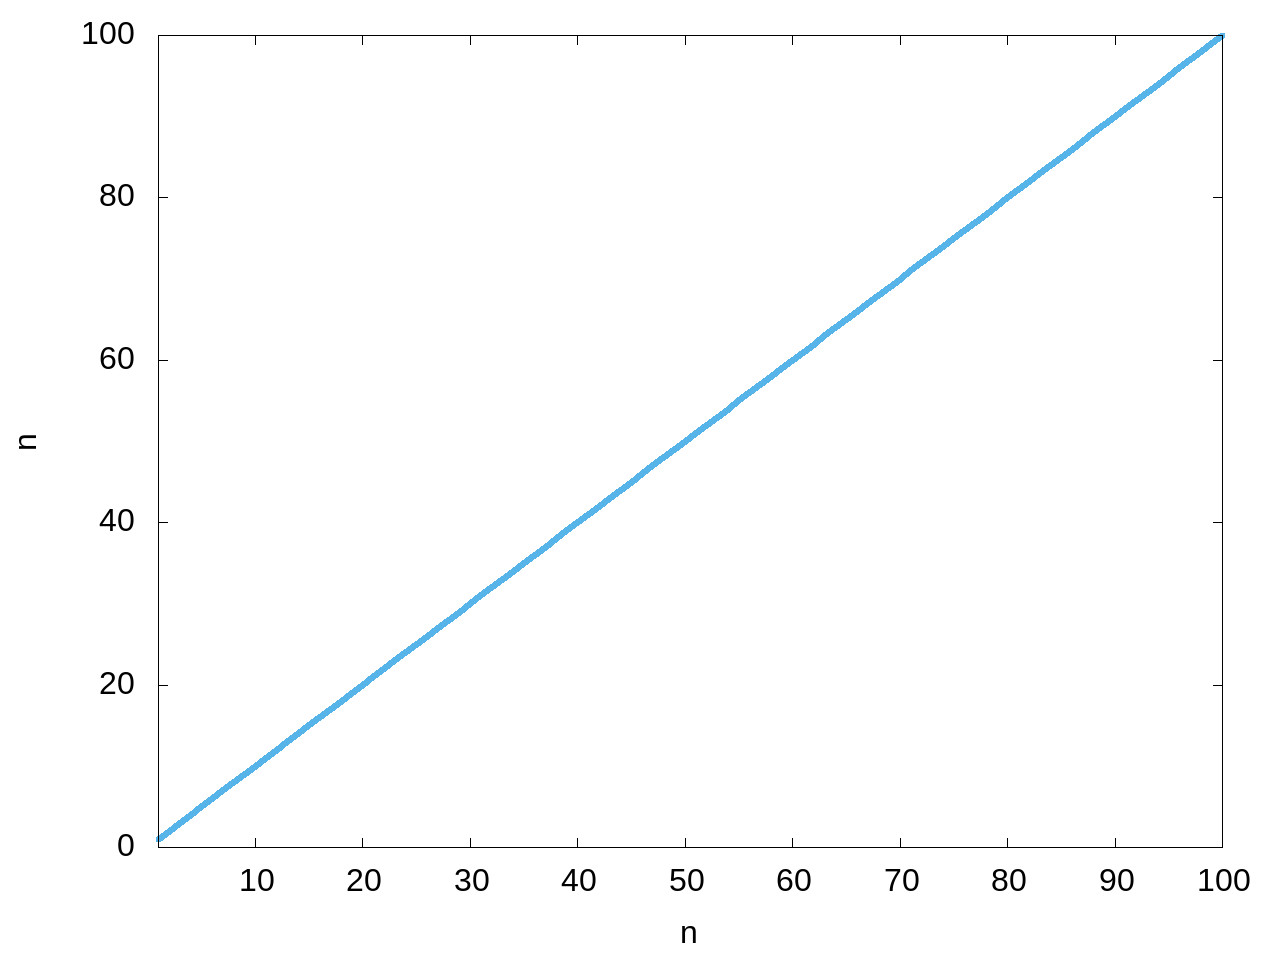
\includegraphics[height=0.5\paperheight]{graficos/n.jpg}
\end{figure}
\end{column}
\begin{column}{0.4\linewidth}
\vspace{5mm}
{\fontsize{0}{4}\selectfont{}\textbf{GNUPLOT:}
\verbatiminput{graficos/n.gnuplot}
}
\end{column}
\end{columns}
\end{frame}

%-------------------------------------------------------
\begin{frame}\frametitle{Função n-log-n: $n \log n$}	
\begin{itemize}
	\item $f(n) = n \log n$
	\item Atribui para uma entrada $n$ o valor de $n$ multiplicado pelo logaritmo de base 2 de $n$
	\item Cresce mais rápido que a função linear e mais devagar que a função quadrática
	\item Exemplo: Algoritmos de ordenação mergesort e heapsort\\\url{http://www.sorting-algorithms.com/}
\end{itemize}
\vspace{-5mm}
\begin{columns}[T]
\begin{column}{0.6\linewidth}
\begin{figure}[h]
	\centering
	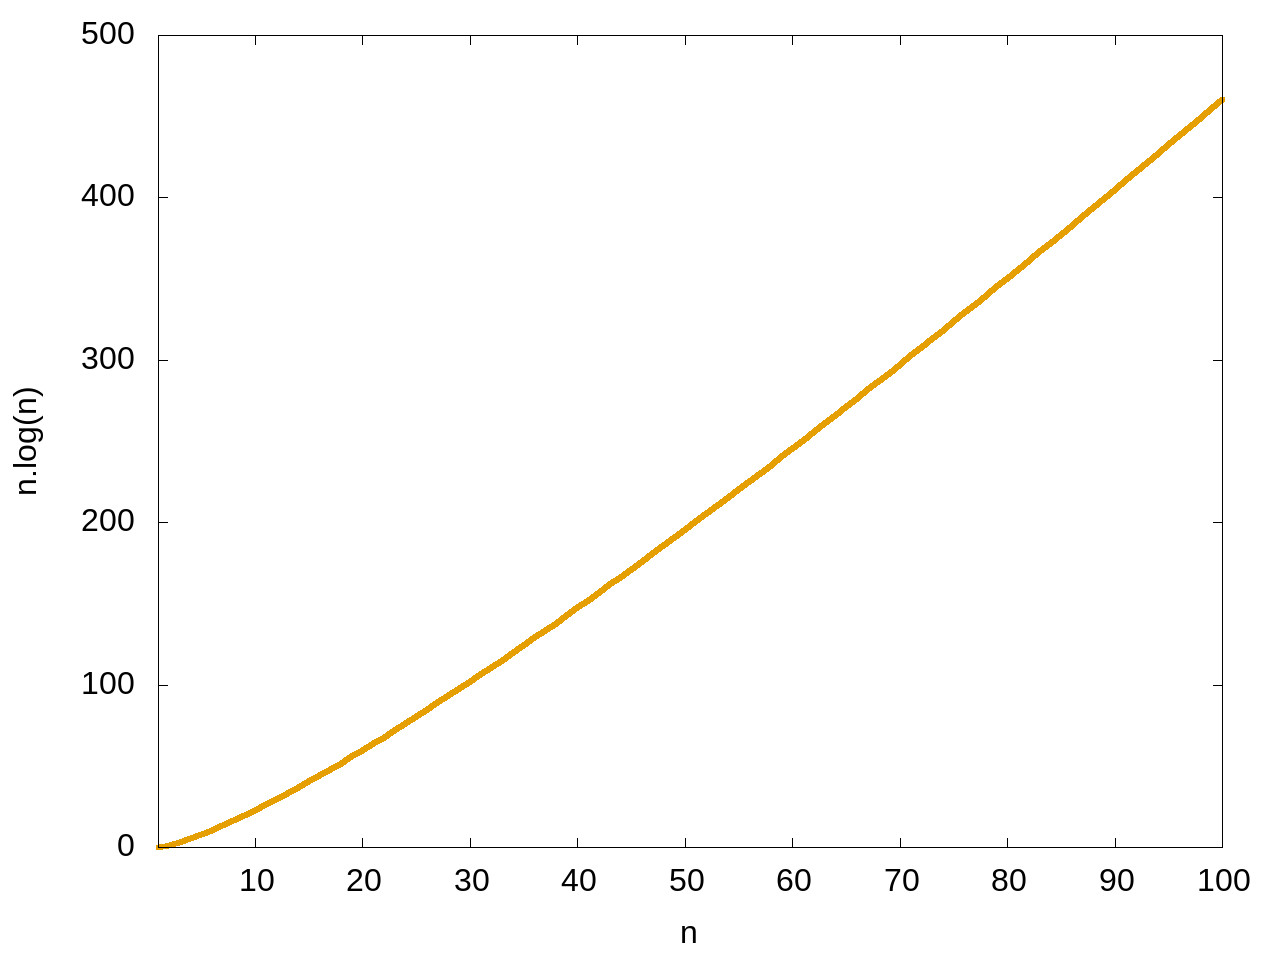
\includegraphics[height=0.5\paperheight]{graficos/n_log_n.jpg}
\end{figure}
\end{column}
\begin{column}{0.4\linewidth}
\vspace{5mm}
{\fontsize{0}{4}\selectfont{}\textbf{GNUPLOT:}
\verbatiminput{graficos/n_log_n.gnuplot}
}
\end{column}
\end{columns}
\end{frame}

%-------------------------------------------------------
\begin{frame}\frametitle{Função Quadrática: $n^2$}
\begin{itemize}
	\item Função polinomial com expoente 2
	\item $f(n) = n^2$
	\item Não cresce de forma abrupta,mas dificultam o uso em problemas grandes.
	\item Exemplo: Ordenação com o algoritmo $bubblesort$
\end{itemize}
\vspace{-5mm}
\begin{columns}[T]
\begin{column}{0.6\linewidth}
\begin{figure}[h]
	\centering
	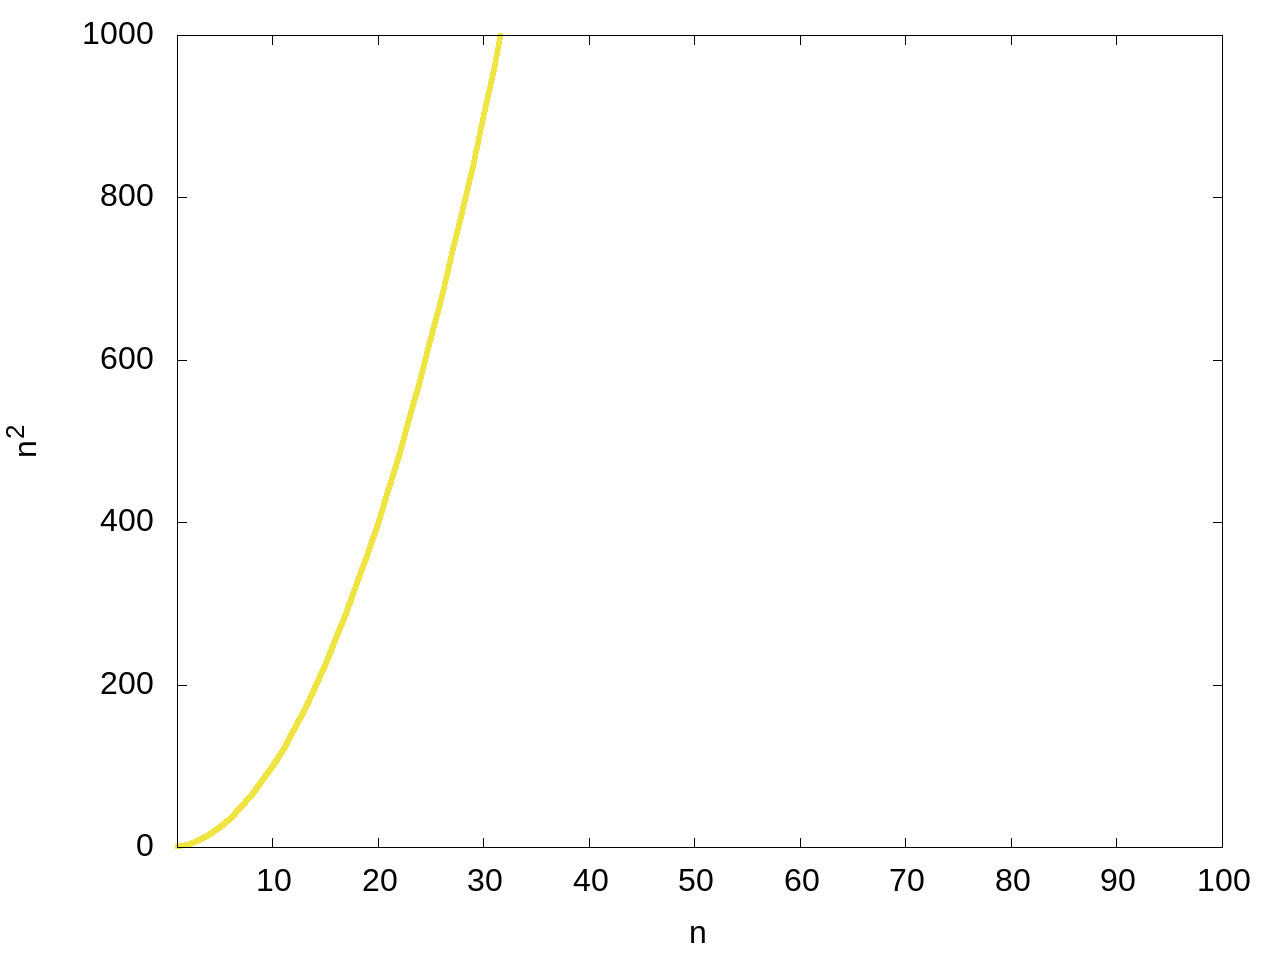
\includegraphics[height=0.5\paperheight]{graficos/n^2.jpg}
\end{figure}
\end{column}
\begin{column}{0.4\linewidth}
\vspace{5mm}
{\fontsize{0}{4}\selectfont{}\textbf{GNUPLOT:}
\verbatiminput{graficos/n^2.gnuplot}
}
\end{column}
\end{columns}
\end{frame}

%-------------------------------------------------------
\begin{frame}\frametitle{Função Cúbica: $n^3$}
\begin{itemize}
	\item Função polinomial com expoente 3
	\item $f(n) = n^3$
	\item Aparece com menos frequência na análise de algoritmos do que as funções constante, linear ou quadrática
	\item Exemplo: multiplicar duas matrizes
\end{itemize}
\vspace{-5mm}
\begin{columns}[T]
\begin{column}{0.6\linewidth}
\begin{figure}[h]
	\centering
	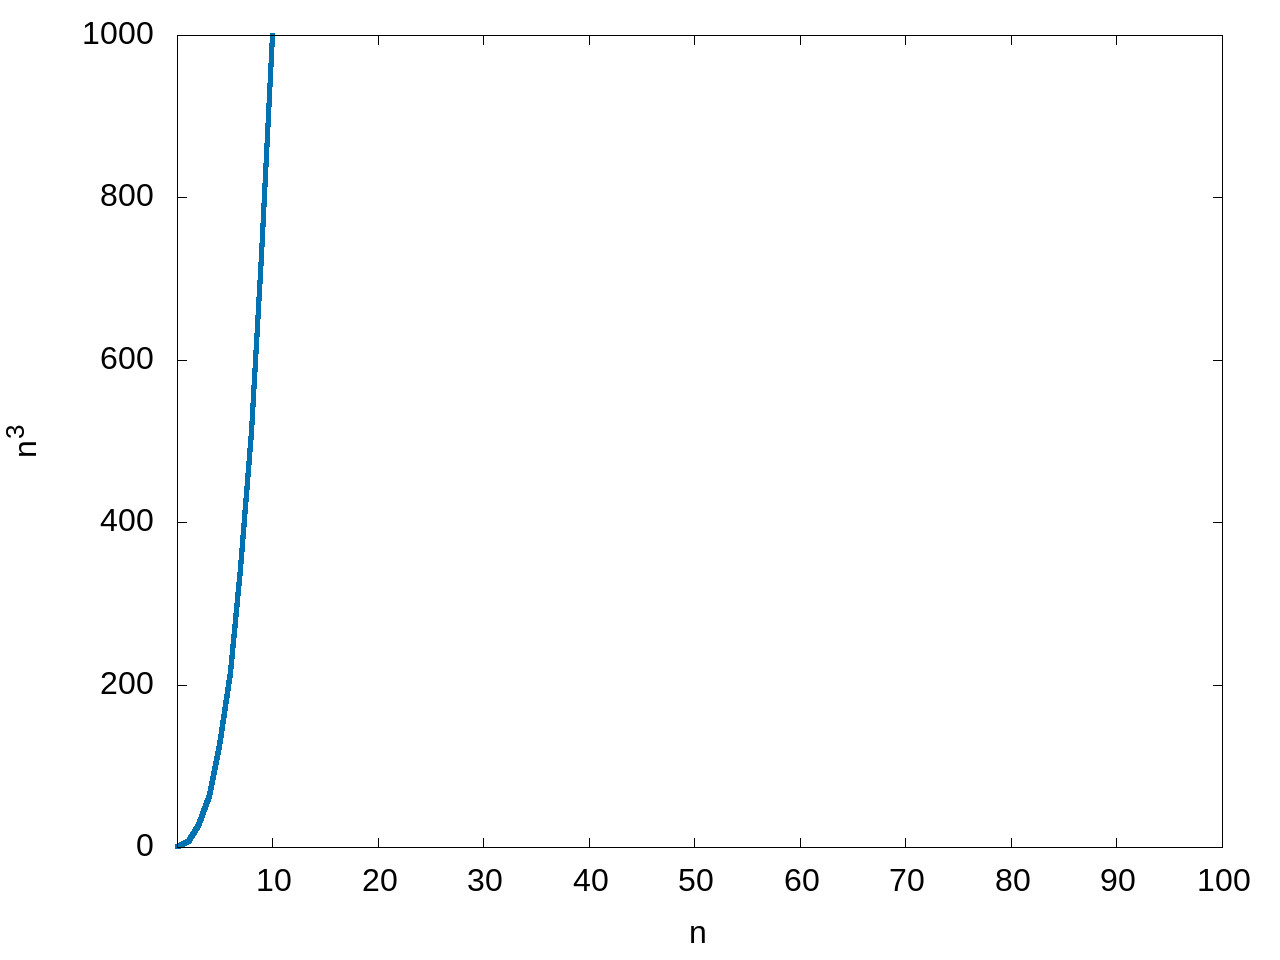
\includegraphics[height=0.5\paperheight]{graficos/n^3.jpg}
\end{figure}
\end{column}
\begin{column}{0.4\linewidth}
\vspace{5mm}
{\fontsize{0}{4}\selectfont{}\textbf{GNUPLOT:}
\verbatiminput{graficos/n^3.gnuplot}
}
\end{column}
\end{columns}
\end{frame}

%-------------------------------------------------------
\begin{frame}\frametitle{Função Exponencial: $a^n$}
\begin{itemize}
	\item Expoente é variável
	\item $f(n) = a^n$
	\item Algoritmos ``ruins'', crescem abruptamente
	\item Aplicável apenas em problemas pequenos.
	\item Exemplos: quebrar senhas com força bruta e listar todos os subconjuntos de um conjunto S
\end{itemize}
\vspace{-5mm}
\begin{columns}[T]
\begin{column}{0.6\linewidth}
\begin{figure}[h]
	\centering
	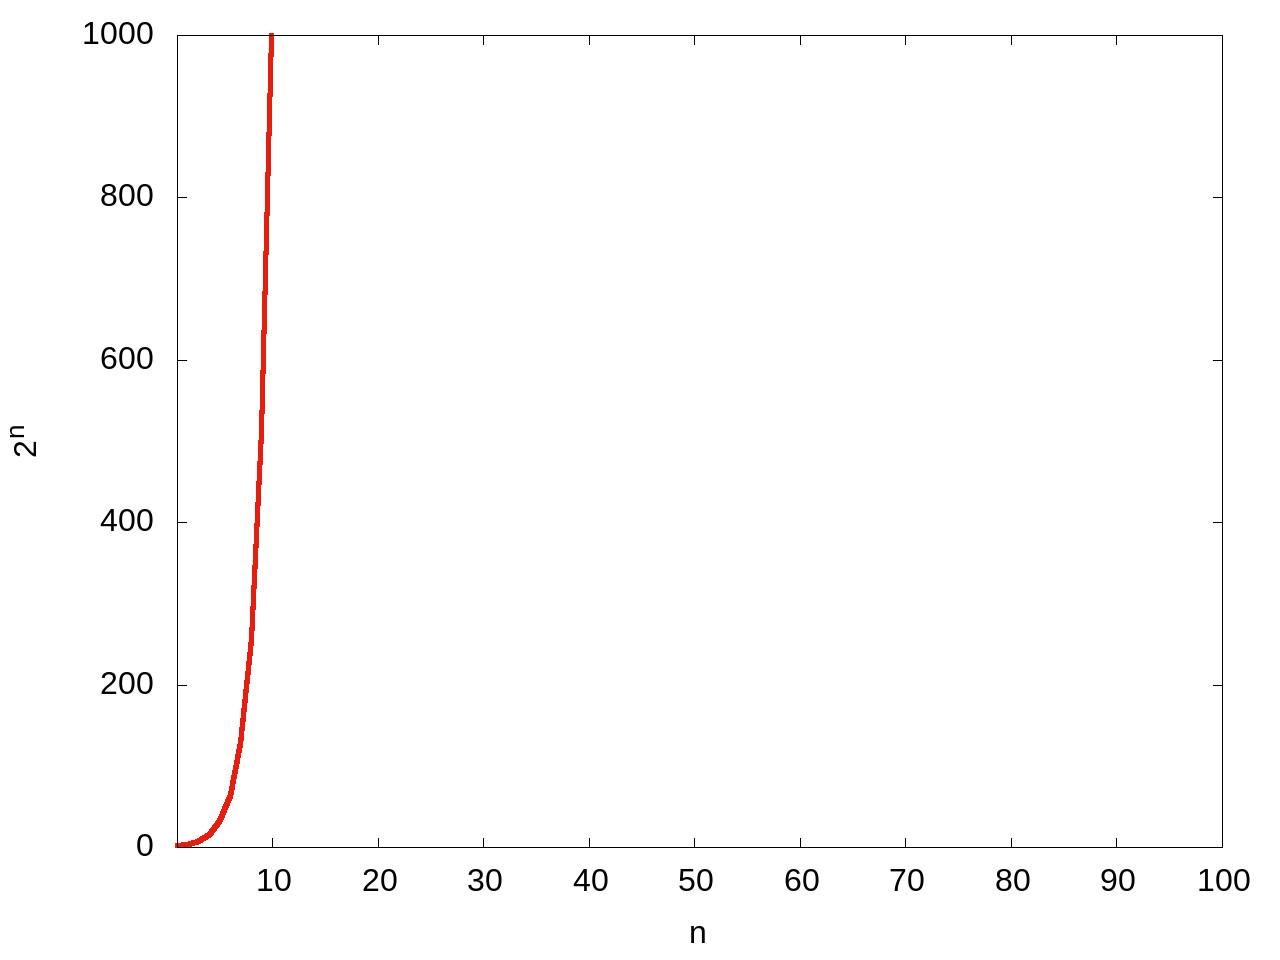
\includegraphics[height=0.5\paperheight]{graficos/2^n.jpg}
\end{figure}
\end{column}
\begin{column}{0.4\linewidth}
\vspace{5mm}
{\fontsize{0}{4}\selectfont{}\textbf{GNUPLOT:}
\verbatiminput{graficos/2^n.gnuplot}
}
\end{column}
\end{columns}
\end{frame}

%-------------------------------------------------------
\begin{frame}\frametitle{Comparativo entre as taxas de crescimento das funções (todas)}
\vspace{-5mm}
\begin{columns}[T]
\begin{column}{0.5\linewidth}
\begin{figure}[h]
	\centering
	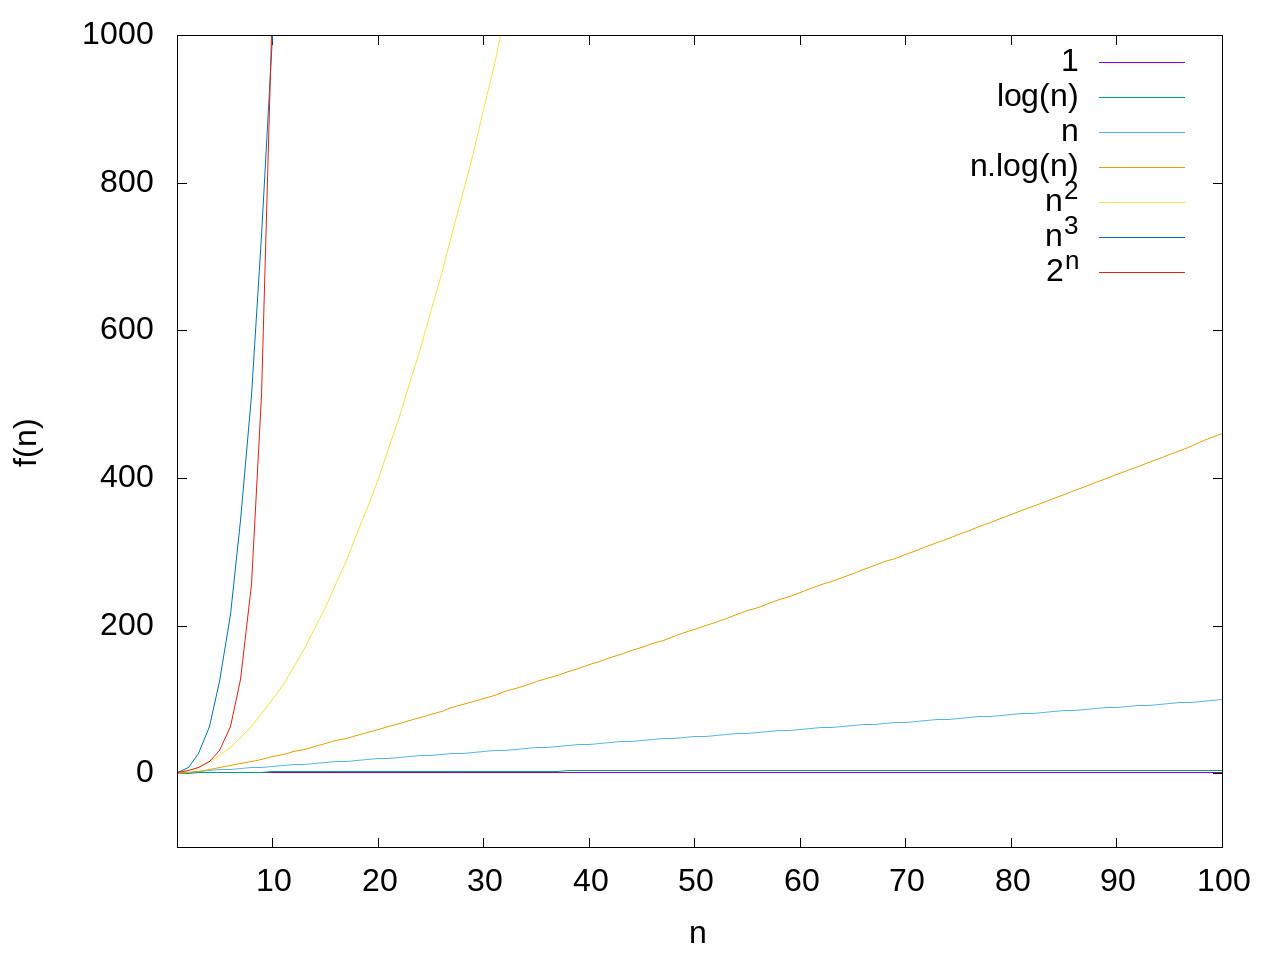
\includegraphics[height=0.65\paperheight]{graficos/todas.jpg}
\end{figure}
\end{column}
\begin{column}{0.5\linewidth}
\vspace{5mm}
{\fontsize{0}{4}\selectfont{}\textbf{GNUPLOT:}
\verbatiminput{graficos/todas.gnuplot}
}
\end{column}
\end{columns}
\end{frame}

%-------------------------------------------------------
\begin{frame}\frametitle{Comparativo entre as taxas de crescimento das funções (grupo 1)}
\vspace{-5mm}
\begin{columns}[T]
\begin{column}{0.5\linewidth}
\begin{figure}[h]
	\centering
	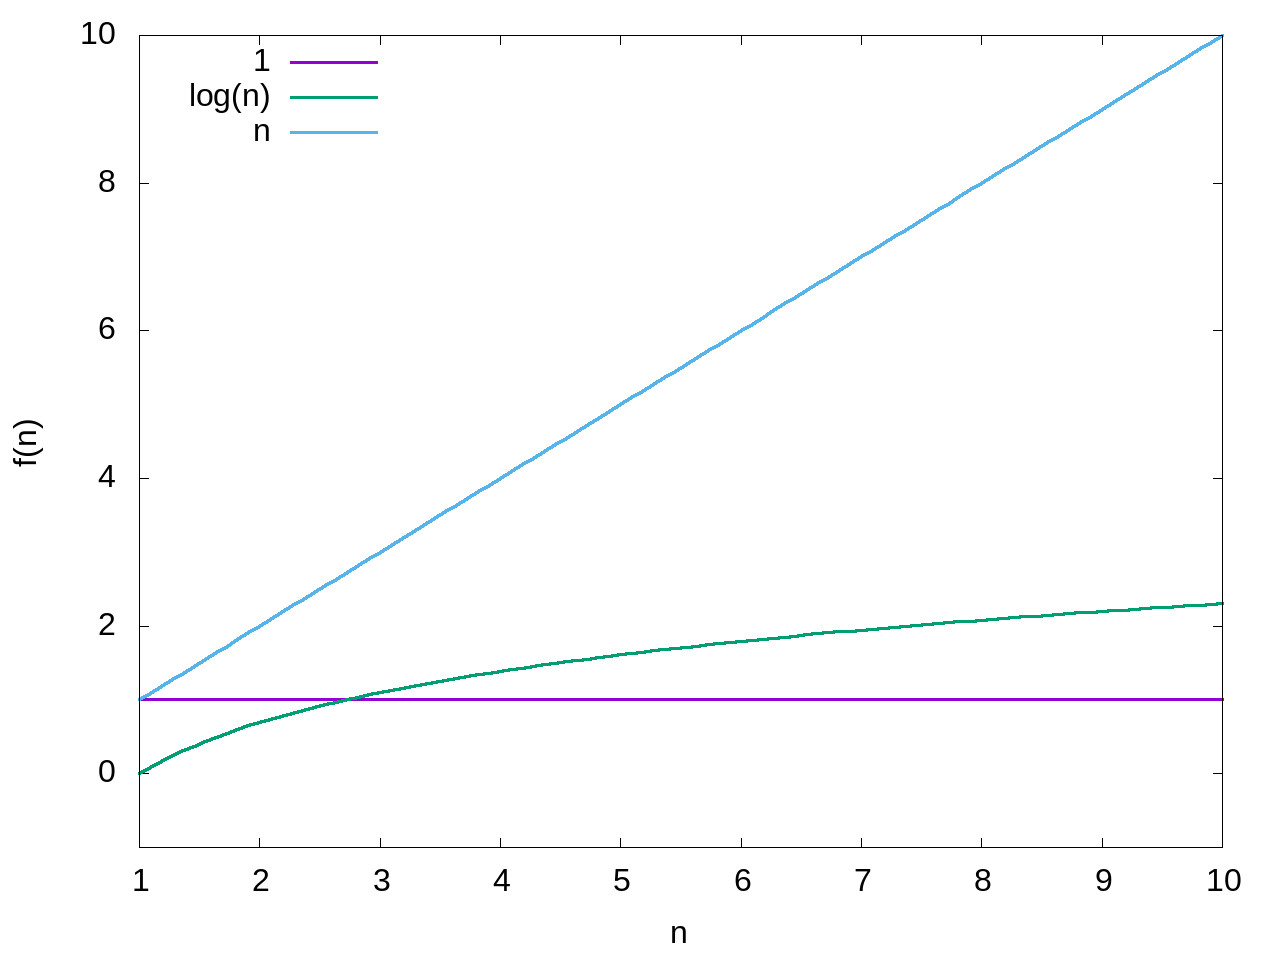
\includegraphics[height=0.65\paperheight]{graficos/grupo1.jpg}
\end{figure}
\end{column}
\begin{column}{0.5\linewidth}
\vspace{5mm}
{\fontsize{0}{4}\selectfont{}\textbf{GNUPLOT:}
\verbatiminput{graficos/grupo1.gnuplot}
}
\end{column}
\end{columns}
\end{frame}

%-------------------------------------------------------
\begin{frame}\frametitle{Comparativo entre as taxas de crescimento das funções (grupo 2)}
\vspace{-5mm}
\begin{columns}[T]
\begin{column}{0.5\linewidth}
\begin{figure}[h]
	\centering
	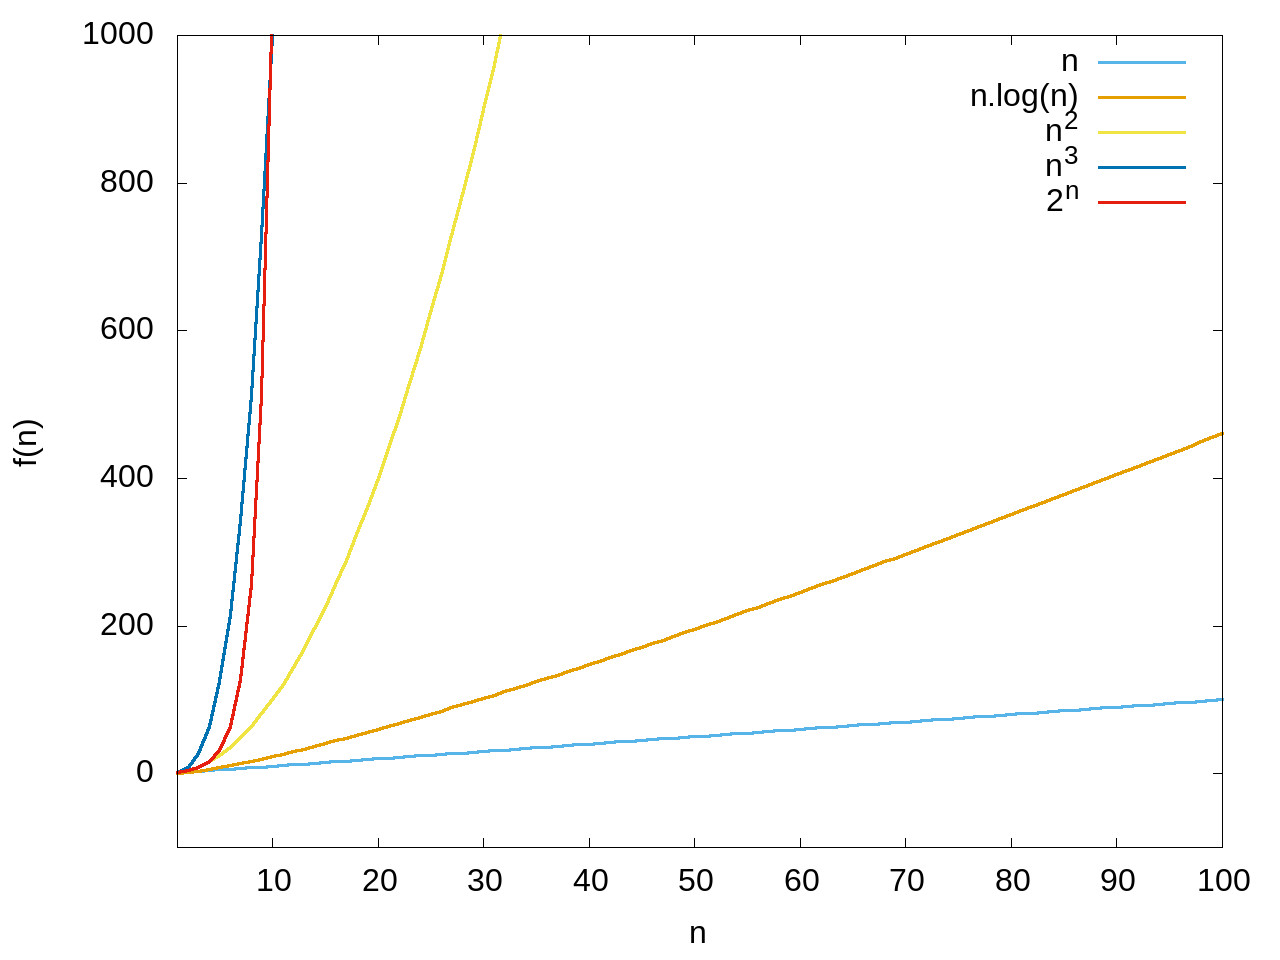
\includegraphics[height=0.65\paperheight]{graficos/grupo2.jpg}
\end{figure}
\end{column}
\begin{column}{0.5\linewidth}
\vspace{5mm}
{\fontsize{0}{4}\selectfont{}\textbf{GNUPLOT:}
\verbatiminput{graficos/grupo2.gnuplot}
}
\end{column}
\end{columns}
\end{frame}

%-------------------------------------------------------
\begin{frame}\frametitle{Comparativo entre as taxas de crescimento das funções (grupo 3)}
\vspace{-5mm}
\begin{columns}[T]
\begin{column}{0.5\linewidth}
\begin{figure}[h]
	\centering
	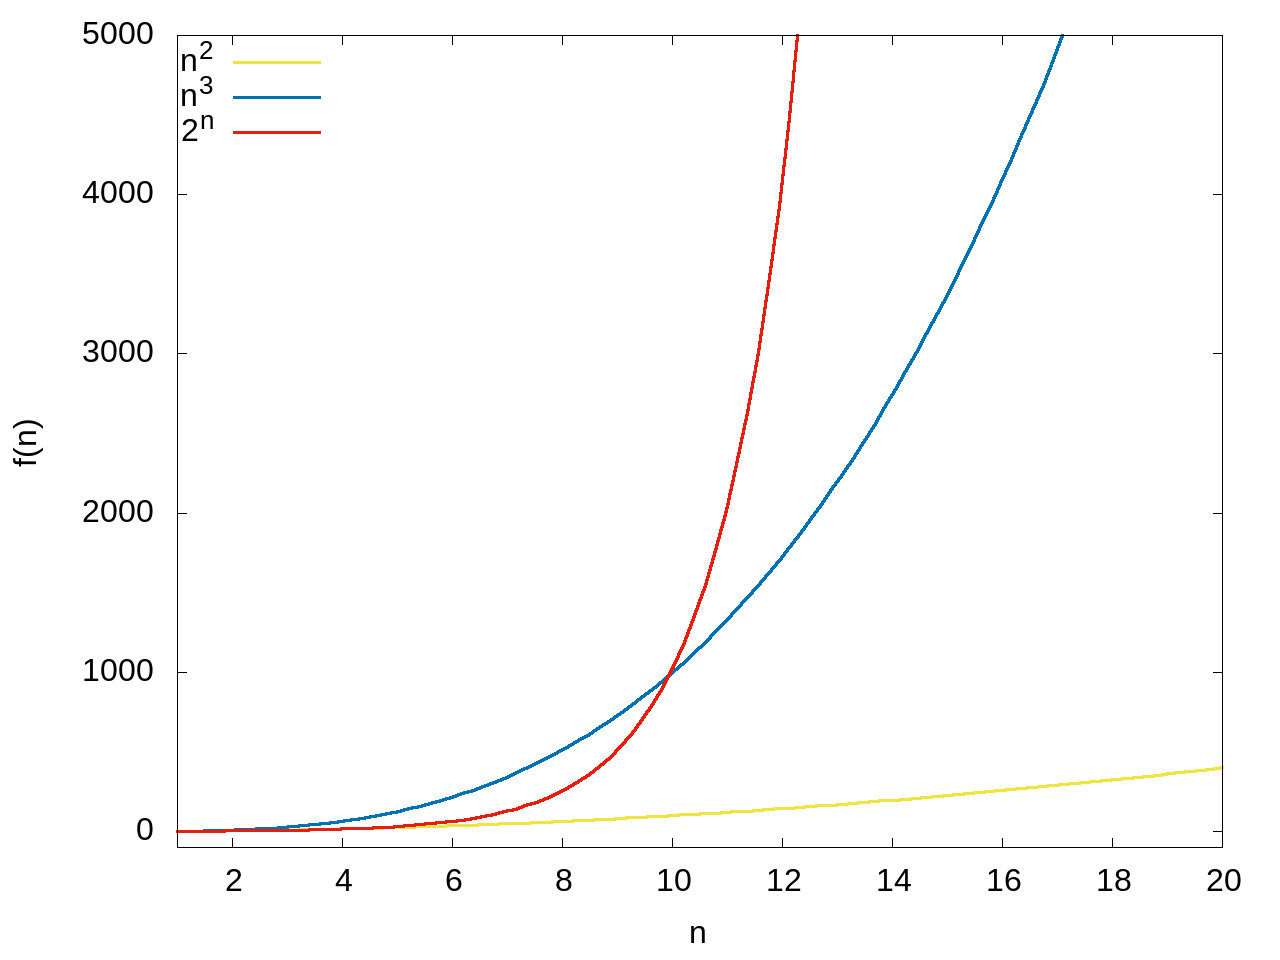
\includegraphics[height=0.65\paperheight]{graficos/grupo3.jpg}
\end{figure}
\end{column}
\begin{column}{0.5\linewidth}
\vspace{5mm}
{\fontsize{0}{4}\selectfont{}\textbf{GNUPLOT:}
\verbatiminput{graficos/grupo3.gnuplot}
}
\end{column}
\end{columns}
\end{frame}

%-------------------------------------------------------
\begin{frame}\frametitle{Funções}
\begin{itemize}
	\item Um problema é dividido em funções/métodos
	\begin{itemize}
		\item Cada função/método tem um ``custo'' diferente
		\item Estes custos são somados para determinar o custo total para solução do problema
	\end{itemize}
\end{itemize}
\end{frame}

\section{Exercícios}

%-------------------------------------------------------
\begin{frame}\frametitle{Exercício 1}
Dois algoritmos para resolver o mesmo problema foram analisados e concluiu-se que eles executam os seguintes números de operações:\\
\begin{itemize}
	\item Algoritmo A: $f_{A}(n) = 2n^2 + 5n$ operações
	\item Algoritmo B: $f_{B}(n) = 500n + 4000$ operações
\end{itemize}
Qual desses algoritmos consiste na melhor solução? Analise o número de operações de cada algoritmo para diferentes valores de $n$ (por exemplo, $n = 10$, $n = 100$, $n = 1000$, etc.)
\end{frame}

%-------------------------------------------------------
\begin{frame}[fragile]\frametitle{Exercício 2}
Analise os algoritmos abaixo e identifique a sua classe de complexidade. Para verificar se a sua resposta está correta, implemente cada algoritmo, teste com diferentes valores de $n$ e gere um gráfico usando o GNUPLOT.
\vspace{-4mm}
\begin{columns}[T]
\begin{column}{0.5\linewidth}
\begin{enumerate}
	\item {\scriptsize\lstinputlisting{contagem/contagem07.c}}
\vspace{-4mm}
	\item {\scriptsize\lstinputlisting{contagem/contagem08.c}}
\end{enumerate}
\end{column}
\begin{column}{0.5\linewidth}
\begin{enumerate}
	\setcounter{enumi}{2}
	\item {\scriptsize\lstinputlisting{contagem/contagem09.c}}
\vspace{-4mm}
	\item {\scriptsize\lstinputlisting{contagem/contagem10.c}}
\end{enumerate}
	\end{column}
\end{columns}
\end{frame}

%-------------------------------------------------------
\begin{frame}[fragile]\frametitle{Exercício 2}
\begin{columns}[T]
\begin{column}{0.5\linewidth}
\begin{enumerate}
	\setcounter{enumi}{4}
	\item {\scriptsize\lstinputlisting{contagem/contagem11.c}}
	\item {\scriptsize\lstinputlisting{contagem/contagem12.c}}
\end{enumerate}
\end{column}
\begin{column}{0.5\linewidth}
\end{column}
\end{columns}
\end{frame}

%-------------------------------------------------------
\begin{frame}\frametitle{Exercício 3}
Faça um algoritmo para o problema abaixo e analise a sua complexidade.\\
~\\
Problema:
\begin{itemize}
	\item Dado um intervalo [1;V]
	\item Determinar quantas sequencias de valores entre 1 e V somam exatamente V
\end{itemize}
Exemplo:
\begin{itemize}
	\item V=15
	\item Sequências
	\begin{itemize}
		\item 1+2+3+4+5
		\item 4+5+6
		\item 7+8
		\item 15
	\end{itemize}
	\item Resposta: 4 sequências de valores somam exatamente 15
\end{itemize}
\end{frame}

\section{Notação $O$}

\newcommand{\sep}{\hspace*{.5em}}
	%-------------------------------------------------------
\begin{frame}\frametitle{Notação $O$}
\begin{itemize}
	\item O número de passos durante a execução de um algoritmo pode variar
	\item Exemplo: ordenar um vetor\\
\noindent $\fbox{2} \sep \fbox{1} \sep \fbox{3} \sep \fbox{4} \sep \fbox{5} \sep \fbox{6}$ \sep x \sep
          $\fbox{6} \sep \fbox{5} \sep \fbox{4} \sep \fbox{3} \sep \fbox{2} \sep \fbox{1}$
	\item Existe o limite superior e o limite inferior para cada algoritmo
	\item Exemplo:\\
\url{https://www.toptal.com/developers/sorting-algorithms/bubble-sort}
\end{itemize}
\end{frame}

%-------------------------------------------------------
\begin{frame}\frametitle{Notação $O$}
\begin{itemize}
	\item Limite inferior
	\begin{itemize}
		\item Menor tempo de execução sobre todas as entradas de tamanho $n$
		\item Exemplo: \emph{Bubble Sort} recebe vetor de entrada quase ordenado
	\end{itemize}
	\item Limite superior
	\begin{itemize}
		\item Maior tempo de execução sobre todas as entradas de tamanho $n$
		\item Exemplo: \emph{Bubble Sort} recebe vetor de entrada ordenado de trás para frente
	\end{itemize}
	\item Caso ``médio''
	\begin{itemize}
		\item Média dos tempos de execução sobre todas as entradas de tamanho n
	\end{itemize}
\end{itemize}
\end{frame}

%-------------------------------------------------------
\begin{frame}\frametitle{Notação $O$}
\begin{itemize}
	\item Tempo cresce conforme a entrada de dados cresce
	\item Determinar o ``tempo médio'' é difícil
	\item Portanto, para análise de algoritmos quase sempre se quer saber o limite superior
	\begin{itemize}
		\item Mais fácil de analisar
		\item Crucial para determinadas aplicações
	\end{itemize}
\end{itemize}
\end{frame}

%-------------------------------------------------------
\begin{frame}\frametitle{Notação $O$}
\begin{itemize}
	\item Importante:
	\begin{itemize}
		\item Concentrar-se na taxa de crescimento do tempo de execução como uma função do tamanho da entrada $n$
	\end{itemize}
	\item Por exemplo:
	\begin{itemize}
		\item No algoritmo que verifica maior número de um arranjo de inteiros, o tempo de execução cresce proporcionalmente a n
		\item Tempo de execução: $n$ vezes um fator constante
	\end{itemize}
\end{itemize}
\end{frame}

%-------------------------------------------------------
\begin{frame}\frametitle{Notação $O$}
\begin{itemize}
	\item Ao ver uma expressão $f(n) = a^n$, normalmente se pensa em valores pequenos
	\begin{itemize}
		\item É o que se consegue resolver
	\end{itemize}
	\item Análise de algoritmos
	\begin{itemize}
		\item Ignora os valores pequenos e concentra-se nos valores enormes de $n$
	\end{itemize}
	\item Para grandes valores de n, as funções $n^2$ , $(3/2)n^2$ , $n^2+100n$, por exemplo, crescem com a mesma velocidade, portanto são equivalentes
\end{itemize}
\end{frame}

%-------------------------------------------------------
\begin{frame}[fragile]\frametitle{Notação $O$}
\vspace{-5mm}
\begin{columns}[T]
\begin{column}{0.5\linewidth}
\begin{figure}[h]
	\centering
	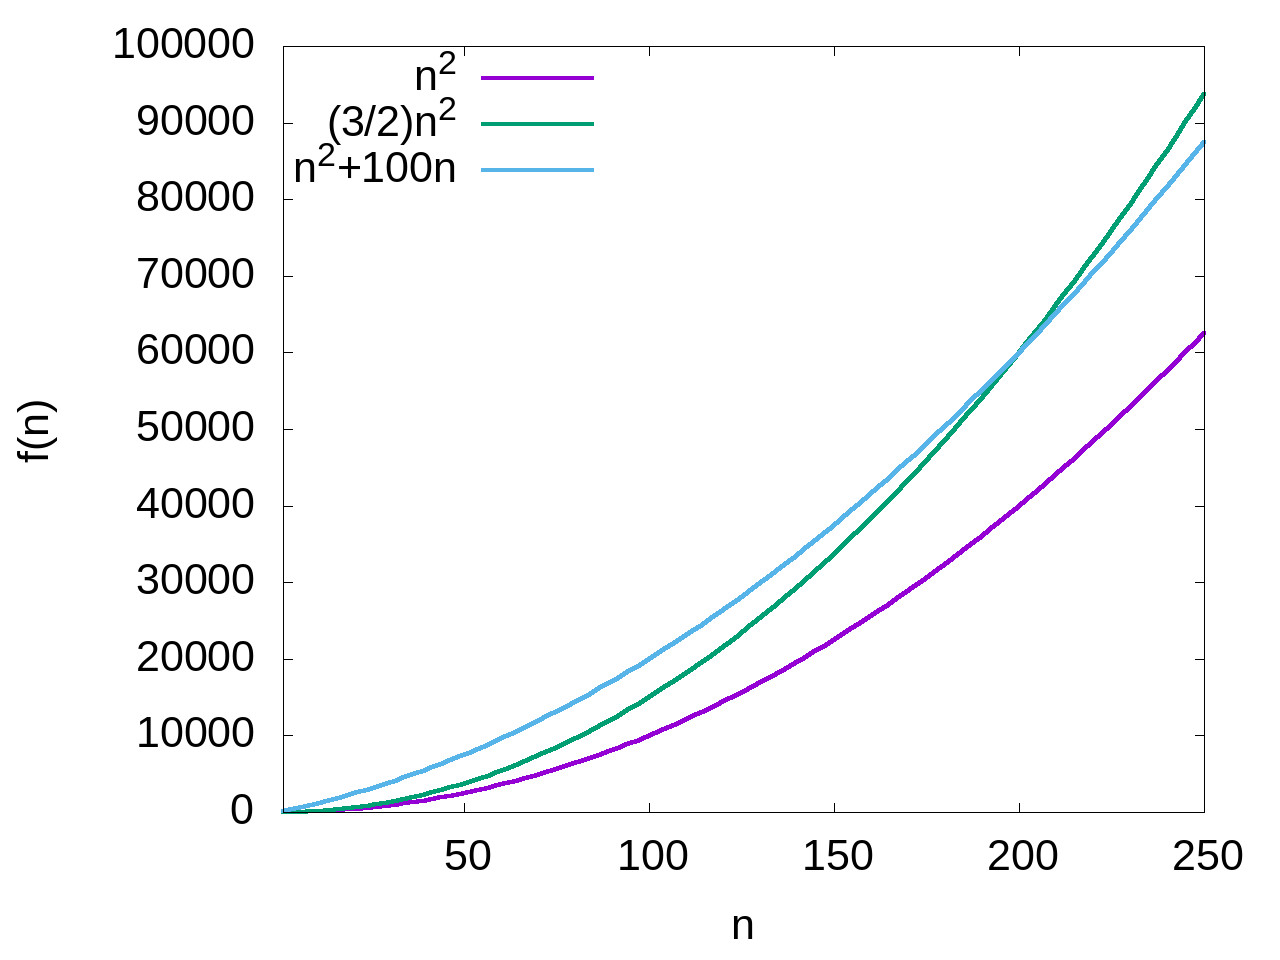
\includegraphics[height=0.65\paperheight]{graficos/grafico2.jpg}
\end{figure}
\end{column}
\begin{column}{0.5\linewidth}
\vspace{5mm}
{\fontsize{0}{4}\selectfont{}\textbf{GNUPLOT:}
\verbatiminput{graficos/grafico2.gnuplot}
}
\end{column}
\end{columns}
\end{frame}

%-------------------------------------------------------
\begin{frame}\frametitle{Notação Assintótica}
\begin{itemize}
	\item Assintótico (Adj.)
	\begin{itemize}
		\item Quando se quer descrever o comportamento quando se aproxima de um limite, ou seja, quando n tende ao infinito
		\item Aquilo que está relativamente próximo
		\item Para todos os valores suficientemente grandes
		\item O comportamento a ser observado em uma função $f(n)$, quando $n$ tende ao infinito
		\item Relativo à Assintota
		\begin{itemize}
			\item (Mat.) linha reta relacionada com uma curva, cuja distância entre elas se torna infinitamente pequena, a partir de determinado ponto
			\item (Fig.) Caminho que se aproxima continuamente de um ideal sem jamais o atingir
		\end{itemize}
	\end{itemize}
	\item Notações
	\begin{itemize}
		\item Notação O
		\item Notação $\Omega$ (ômega)
		\item Notação $\Theta$ (\emph{theta})
	\end{itemize}
\end{itemize}
\end{frame}

%-------------------------------------------------------
\begin{frame}\frametitle{Notação $O$}
\begin{itemize}
	\item Sejam $f(n)$ e $g(n)$ funções mapeando inteiros não negativos em números reais
	\item Diz-se que $f(n)$ é $O(g(n))$ se existe uma constante real $c > 0$ e uma constante inteira $n_0 \ge 1$ tais que
$f(n) \le cg(n)$, para todo inteiro $n \ge n_0$
\begin{figure}[h]
	\centering
	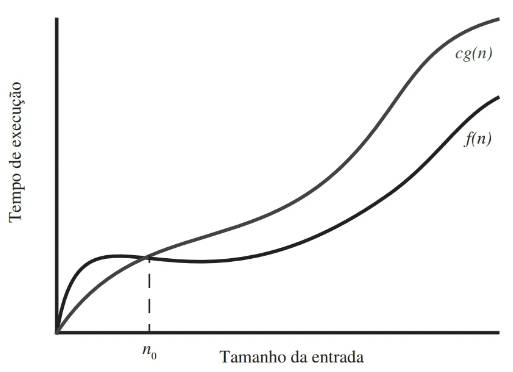
\includegraphics[height=0.5\paperheight]{imagens/grafico_fx_gx.jpg}
\end{figure}
\end{itemize}
\end{frame}

%-------------------------------------------------------
\begin{frame}\frametitle{Notação $O$}
\begin{itemize}
	\item Notação O:
	\begin{itemize}
		\item $f(n)$ é \textbf{O} de $g(n)$
		\item $f(n)$ é \textbf{da ordem} de $g(n)$
	\end{itemize}
	\item $f(n)=O(g(n))$
	\begin{itemize}
		\item Significa que $g(n)$ cresce mais (ou da mesma forma que) a função $f(n)$ à medida que $n$ cresce para o infinito
		\item Para isso, pode ser preciso multiplicar $g(n)$ por uma constante
	\end{itemize}
	\item Notação O é usada para
	\begin{itemize}
		\item \textbf{Caracterizar o tempo de execução} e limites espaciais em função de um parâmetro $n$ que varia de problema para problema
	\end{itemize}
\end{itemize}
\end{frame}

%-------------------------------------------------------
\begin{frame}\frametitle{Notação $O$}
\begin{itemize}
	\item Exemplo: algoritmo para encontrar o maior elemento de um arranjo de inteiros
	\begin{itemize}
		\item $n$ representa o número de elementos no arranjo
		\item Usando a notação $O$ se pode afirmar (independente do computador que será usado):
		\begin{itemize}
			\item Este algoritmo executa em tempo $O(n)$
		\end{itemize}
		\item Justificativa:
		\begin{itemize}
			\item O número de operações primitivas executadas pelo algoritmo é constante em cada iteração
			\item Pode-se dizer que o tempo de execução do algoritmo para uma entrada de tamanho $n$ é no máximo uma constante, vezes $n$
		\end{itemize}
	\end{itemize}
\end{itemize}
\end{frame}

%-------------------------------------------------------
\begin{frame}\frametitle{Propriedades da notação $O$}
\begin{itemize}
	\item Permite ignorar os fatores constantes e os termos de menor ordem, focando nos principais componentes da função que afetam seu crescimento
	\item Se $f(n)$ é um polinômio de grau $d$, isto é,
\[f(n) = a_0 + a_{1}n + ... + a_{d}n^{d}\]
e $a_d > 0$, então $f(n)$ é $O(n^{d})$
	\item Deve-se descrever a função O em termos simples
\end{itemize}
\end{frame}

%-------------------------------------------------------
\begin{frame}\frametitle{Propriedades da notação $O$}
\begin{itemize}
	\item Portanto, o termo de mais alto grau em um polinômio é o termo que determina a taxa de crescimento assintótico do polinômio
	\item Exemplos:
	\begin{itemize}
		\item $5n^2 + 3n\log{n} + 2n + 5$ é $O(n^2)$
		\item $20n^3 + 10n\log{n} + 5$ é $O(n^3)$
		\item $3\log{n} + 2$ é $O(\log{n})$
		\item $2^{n+2}$ é $O(2^n)$
		\item $2n + 100\log{n}$ é $O(n)$
	\end{itemize}
\end{itemize}
\end{frame}

%-------------------------------------------------------
\begin{frame}\frametitle{Notação $O$}
\begin{itemize}
	\item As sete funções apresentadas são as mais usadas em conjunto com a notação $O$\\
$1$, $\log{n}$, $n$, $n\log{n}$, $n^2$, $n^3$, $a^n$
	\item Caracterizam os tempos de execução e consumo de memória dos algoritmos
	\item Os nomes destas funções são usados para referenciar o tempo de execução
	\item Exemplos:
	\begin{itemize}
		\item  Algoritmo que executa no limite superior em tempo $4n^2 + n\log{n}$ é um algoritmo de tempo quadrático, pois executa em tempo $O(n^2)$
		\item Algoritmo que executa no limite superior em $5n + 20\log{n} + 4$ é um algoritmo de tempo linear, ou seja, $O(n)$
	\end{itemize}
	\end{itemize}
\end{frame}

\section{Notação $\Omega$ e Notação $\Theta$}

%-------------------------------------------------------
\begin{frame}\frametitle{Notação $\Omega$ e Notação $\Theta$}
\begin{itemize}
	\item Notação $O$\\
	Maneira assintótica de dizer que uma função é ``menor que ou igual a'' outra função
	\item Notação $\Omega$\\
	Maneira assintótica de dizer que uma função cresce a uma taxa que é ``maior ou igual a'' outra função
	\item Notação $\Theta$\\
	Permite dizer que duas funções crescem à mesma taxa
	\end{itemize}
\end{frame}

%-------------------------------------------------------
\begin{frame}\frametitle{Notação $\Omega$}
\begin{itemize}
	\item Sejam $f(n)$ e $g(n)$ funções mapeando inteiros não negativos em números reais
	\item Diz-se que $f(n)$ é $\Omega(g(n))$ se $g(n)$ é $O(f(n))$, ou seja, se existe uma constante real $c > 0$ e uma constante inteira $n_0 \ge 1$ tais que $f(n) \ge cg(n)$, para todo inteiro $n \ge n_0$
	\item Permite dizer que uma função é assintoticamente maior que ou igual a outra, exceto por um fator constante
	\item Se diz que $f(n)$ \textbf{é ômega de} $g(n)$
	\item Exemplo: $3n\log{n} + 2n$ é $\Omega(n\log{n})$
\end{itemize}
\end{frame}

%-------------------------------------------------------
\begin{frame}\frametitle{Notação $\Theta$}
\begin{itemize}
	\item Diz-se que $f(n)$ é $\Theta(g(n))$, se $f(n)$ é $O(g(n))$ e $f(n)$ é $\Omega(g(n))$, ou seja, existem constantes reais $c' > 0$ e $c'' > 0$ e uma constante inteira $n_0 \ge 1$ tais que $c'g(n) \le f(n) \le c''g(n)$, para $n \ge n_0$
	\item Se diz que $f(n)$ \textbf{é theta} de $g(n)$
	\item Exemplo: $3n\log{n} + 4n + 5 \log{n}$ é $\Theta(n\log{n})$
\end{itemize}
\end{frame}

%-------------------------------------------------------
\begin{frame}\frametitle{Exemplo de gráficos das notações $O$, $\Omega$ e $\Theta$}
\begin{itemize}
	\item Notação $\Theta$ limita uma função entre valores constantes
	\item Notação $O$ dá um limite superior para uma função dentro de um valor constante
	\item Notação $\Omega$ dá um limite inferior para uma função dentro de um valor constante
		\end{itemize}
\begin{figure}[h]
	\centering
	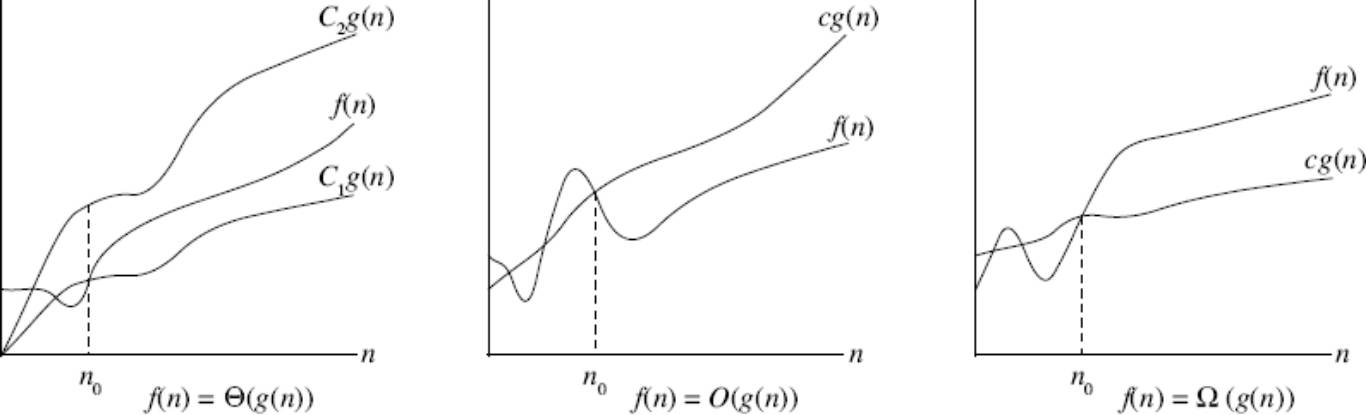
\includegraphics[height=0.5\paperheight]{imagens/notacoes.jpg}
\tiny{Fonte: Cormen \emph{et al.} (2012)}
\end{figure}
\end{frame}

\section{Análise assintótica}

%-------------------------------------------------------
\begin{frame}\frametitle{Análise assintótica}
\begin{itemize}
	\item Suponha dois algoritmos, A e B, para resolver um mesmo problema
	\begin{itemize}
		\item A tem um tempo de execução $O(n)$
		\item B tem um tempo de execução $O(n^2)$
		\item Qual deles é melhor?
		\item A é assintoticamente melhor que B
	\end{itemize}
\end{itemize}
\end{frame}

%-------------------------------------------------------
\begin{frame}\frametitle{Análise assintótica}
\begin{itemize}
	\item Pode-se usar a notação $O$ para ordenar classes de funções por seu crescimento assintótico\\
$1$ ~ ~ $\log{n}$ ~ ~ $n$ ~ ~ $n\log{n}$ ~ ~ $n^2$ ~ ~ $n^3$ ~ ~ $2^n$
\end{itemize}
\begin{figure}[h]
	\centering
	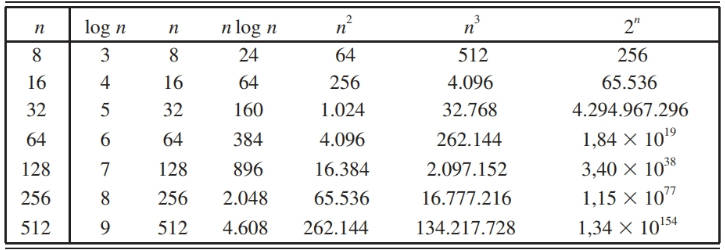
\includegraphics[height=0.5\paperheight]{imagens/tabela.jpg}
\end{figure}
\end{frame}

%-------------------------------------------------------
\begin{frame}\frametitle{Análise assintótica}
\begin{itemize}
	\item Para analisar algoritmos com a notação $O$, o mais apropriado é dizer:\\
$f(n)$ é $O(g(n))$,\\
ou\\
$f(n) \in O(g(n))$
\end{itemize}
\end{frame}

%-------------------------------------------------------
\begin{frame}\frametitle{O que é um algoritmo rápido?}
\begin{itemize}
	\item Em geral, um algoritmo executando em tempo $O(n\log{n})$, com um fator constante razoável, pode ser considerado eficiente
	\item Até um método $O(n^2)$ pode ser suficientemente rápido em alguns contextos ($n$ pequeno)
	\item Algoritmo executando em tempo $O(2^n)$ dificilmente pode ser considerado eficiente
\end{itemize}
\end{frame}

%-------------------------------------------------------
\begin{frame}\frametitle{Análise assintótica}
\begin{itemize}
	\item Notações $O$, $\Omega$ e $\Theta$ fornecem uma linguagem conveniente para análise de estruturas de dados e algoritmos
	\begin{itemize}
		\item Permitem a concentração nos aspectos gerais, em vez dos detalhes
	\end{itemize}
\end{itemize}
\end{frame}

%-------------------------------------------------------
\begin{frame}[fragile]\frametitle{Exercício 1} % Fonte: https://create.kahoot.it/details/2e37a282-4d9d-4902-8afc-9b827ed393fc
Qual a complexidade do algoritmo abaixo?
{\scriptsize
\begin{verbatim}
v[1..N] : inteiro
maximo = 0
for (i=1; i<=n; ++i)
    sum = 0   // sum = somatorio de x[i..j]
    for (j = i; j <= n; ++j)
        sum += x[j]
    maximo = max(maximo,sum)
\end{verbatim}
}
\begin{enumerate}[A]
	\item $O(n)$
	\item $O(n^2)$ % CERTA
	\item $O(n \log 2n)$
	\item $O(2n)$
\end{enumerate}
\end{frame}

%-------------------------------------------------------
\begin{frame}[fragile]\frametitle{Exercício 2} % Fonte: https://create.kahoot.it/details/2e37a282-4d9d-4902-8afc-9b827ed393fc
Qual a complexidade do algoritmo abaixo?
{\scriptsize
\begin{verbatim}
int busca(v[1..N] : inteiro, elem : inteiro)
    for (i = 1; i <= n; i++)
        if (elem == v[i])
           return i // elemento encontrado no indice i
    return -1  // elemento NAO encontrado
\end{verbatim}
}
\begin{enumerate}[A]
	\item $O(n)$ % CERTA
	\item $O(n^2)$
	\item $O(n \log 2n)$
	\item $O(2n)$
\end{enumerate}
\end{frame}

%-------------------------------------------------------
\begin{frame}[fragile]\frametitle{Exercício 3} % Fonte: P1 (2023/1) - Iaçanã Ianiski Weber
Analise os trechos de algoritmos abaixo e identifique suas respectivas classes de complexidade.

\begin{columns}[T]
\begin{column}{0.5\linewidth}
\begin{enumerate}
	\item \textbf{Algoritmo I:}
{\scriptsize
\begin{verbatim}
for (i=0; i < n; i++)
    for (j=0; j < n; j++)
         a += i*3 + aa[i][j];
\end{verbatim}
}
	\item \textbf{Algoritmo II:}
{\scriptsize
\begin{verbatim}
for (i=1; i < n; i=i+i)
    b = b >> i;
\end{verbatim}
}
	\item \textbf{Algoritmo III:}
{\scriptsize
\begin{verbatim}
for (i=0; i < n; i++)
    for (j=0; j < n; j++)
        for (k=0; k < n; k++)
            c += i + j + k;
\end{verbatim}
}
\end{enumerate}
\end{column}
\begin{column}{0.5\linewidth}
\begin{enumerate}
	\setcounter{enumi}{3}
	\item \textbf{Algoritmo IV:}
{\scriptsize
\begin{verbatim}
for (i=0; i < n; i++)
    for (j=i; j < i+5; j++)
        for (k=0; k < n; k++)
            d++;
\end{verbatim}
}
	\item \textbf{Algoritmo V:}
{\scriptsize
\begin{verbatim}
for (i=0; i < 127; i++)
    for (j = 0; j < 127; j++)
        e[i][j] = 0;
\end{verbatim}
}
\end{enumerate}
\end{column}
\end{columns}
\end{frame}

%-------------------------------------------------------
\begin{frame}[fragile]\frametitle{Exercício 4} % Fonte: P1 (2023/1) - Iaçanã Ianiski Weber
Considere as seguintes funções:
\[ f_1(n) = O(n) \qquad f_2(n) = O(\log{n}) \qquad f_3(n) = O(2^n) \qquad f_4(n) = O(n^2) \]
A sequência que apresenta as funções acima ordenadas, pela sua taxa de crescimento, de forma crescente é:
\begin{enumerate}[A]
	\item $f_2$ -- $f_1$ -- $f_4$ -- $f_3$ % CERTA
	\item $f_3$ -- $f_4$ -- $f_1$ -- $f_2$
	\item $f_1$ -- $f_3$ -- $f_2$ -- $f_4$
	\item $f_1$ -- $f_2$ -- $f_3$ -- $f_4$
	\item $f_2$ -- $f_1$ -- $f_3$ -- $f_4$
\end{enumerate}
\end{frame}

%-------------------------------------------------------
\begin{frame}[fragile]\frametitle{Exercício 5} % Fonte: P1 (2023/1) - Iaçanã Ianiski Weber
Qual a notação $O$ dos algoritmos que têm as seguintes taxas de crescimento assintóticas?
\begin{enumerate}[a]
	\item $3n\log{n} + 2n + 5$      % $O(n)$
	\item $1000n\log{n} + 15n^3$    % $O(n^3)$
	\item $8 \log{n} + n$           % $O(n)$
	\item $500n^5 + 2n$             % $O(2^n)$
	\item $10\log{n} + 1521$        % $O(\log{n})$
	\item $3n + 4500n$              % $O(n)$
	\item $3n + 753\log{n} + 4$     % $O(n)$s
\end{enumerate}
	\end{frame}

%=======================================================
\section{Créditos}

%-------------------------------------------------------
\begin{frame}\frametitle{Créditos}
\begin{itemize}
	\item Estas lâminas contêm trechos de materiais criados e disponibilizados pelos professores Isabe Harb Manssour e Iaçanã Ianiski Weber.
\end{itemize}
\end{frame}

%-------------------------------------------------------
\end{document}

